\documentclass[twocolumn,smallextended,runningheads]{svjour3}
\raggedbottom
\usepackage{SpringerLarge}  % patched locally to use Computer Modern (texlive-basic compat)

\usetikzlibrary{positioning, arrows.meta, fit}

\newcommand{\sttttablefont}{\footnotesize}

\smartqed  % flush right qed marks, e.g. at end of proof
\journalname{}

\begin{document}

\title{Region-Relative Verification of TinyTaxiNet Using Marabou~2.0}
\titlerunning{Region-Relative Verification of TinyTaxiNet}

\author{Jireh Katebe}
\authorrunning{J.\,Katebe}

\institute{J.\,Katebe \at
  Vanderbilt University, Nashville, TN 37235, USA \\
  \email{katebejireh@gmail.com}
}

\date{}

% ============================================================
\abstract{%
In formal verification of image-based neural networks, a SAT/UNSAT verdict is exact only for the input region encoded for the solver, and constructing that region is a consequential modeling choice. This paper treats input-region selection as an explicit experimental variable. We introduce a reusable Marabou workflow that reruns a fixed property family across six input abstractions, tags each verdict with the region that produced it, and audits recovered counterexamples against dataset-support signals. Evaluated on TinyTaxiNet, an open-source runway centerline-tracking surrogate, the workflow separates three verdict patterns. First, a too-loose region admits pixel combinations outside the released images: one heading-error violation disappears once the mean-centering constraint satisfied by every released image, $\mathrm{mean}(x){=}0.5$, is enforced. Second, several verdict changes are driven by dimensionality rather than by the learned region itself: two centered cross-track output-bound queries that become UNSAT inside an 8D autoencoder decoder-box also become UNSAT inside matched random 8D affine regions, and a local-robustness verification rate that rises from 186/893 anchors to 847/893 under 8D local PCA is matched or exceeded by random subspaces of the same dimension. A dimension sweep shows that data-aligned directions begin to matter beyond $d\approx16$, where PCA regions recover cross-track counterexamples that random subspaces at the same scale mostly miss. Third, one failure mode is persistent: a wrong-sign cross-track error survives every tested region tightening and is observed directly on images in the released simulator dataset. Instantiations on MNIST, VNN-COMP \texttt{mnist\_fc}, and LARD V2 runway imagery reproduce the dimensionality pattern under matched random controls. The released artifact packages the region constructors, tagged-query execution, and witness audits as a reusable module.%
}

\keywords{Neural network verification \and Marabou \and Image-based perception \and Input-region tagging \and Witness audit \and Completeness-realism trade-off \and TinyTaxiNet \and MNIST}

\maketitle

% ============================================================
\section{Introduction}\label{sec:introduction}

In formal verification of image-based neural networks, solver verdicts are meaningful only with respect to the input region presented to the verifier. For piecewise-linear image networks, per-pixel boxes and $L_\infty$ balls are straightforward to express in Marabou because they become lower and upper bounds on input variables, but they can contain pixel combinations that are far outside the image structure induced by a camera and preprocessing pipeline. Learned, local, or analytically constrained regions move in the opposite direction: they reduce loose pixel combinations seen by the solver, but their guarantees hold only over the fitted or encoded support model. Prior work exposes this issue through runway image-perturbation studies, generator-composed verification, analytic observation models, and surveys of vision-based autonomous-system verification~\cite{elboher2024runway,katz2022,yang2022tiler,estornell2025visual,mitra2024visionsurvey}. This paper treats input-region construction as an explicit verification variable.

We present a region-tagged verification workflow for Marabou (Fig.~\ref{fig:workflow}). Each SAT/UNSAT verdict is reported with the input region that produced it, the same property family is rerun under multiple region tags, and recoverable SAT witnesses are audited using classifier probability, nearest-real-image $L_2$ distance, and per-pair Lipschitz violation fraction. A separate closed-form input-Jacobian and saturating-perturbation diagnostic accounts for postcondition effects, so output-axis asymmetries are not mistaken for architectural robustness.

The reusable artifact centers on the workflow implementation. The \texttt{region\_audit.py} module packages region constructors, tagged query execution, and witness-audit signals for flattened image-input ReLU networks. A new instantiation supplies the network reader, data loader, subset rules, neighbor rule, and calibration data; the module then attaches the selected region, runs the query, serializes the region tag and parameters, and scores recovered witnesses against a same-domain baseline.

A practitioner using the workflow selects one or more region constructions appropriate for the verification question, reruns the same property family under those regions, and compares the tagged verdicts. Recovered SAT witnesses are then audited against dataset-support signals before being treated as candidate failure modes. The released module automates these steps while leaving the solver and property specification explicit.

This distinction matters in practice: an untagged SAT witness can be mistaken for a network failure when it is supported mainly by a broad abstraction, while a witness that survives tighter regions and appears in data calls for a different engineering response.

\begin{table*}[t]
\centering
\sttttablefont
\setlength{\tabcolsep}{4pt}
\begin{tabular}{p{0.20\textwidth}p{0.30\textwidth}p{0.40\textwidth}}
\toprule
Evidence block & Role & Claim scope \\
\midrule
TinyTaxiNet & Main P1/P3/P4 case study & Region-relative verdict interpretation \\
MNIST MLP & Second-model protocol check & Workflow transfer; domain-specific audit thresholds \\
VNN-COMP \texttt{mnist\_fc} & External image classifier & Bounded low-dimensional removal on a non-authored network \\
LARD V2 & External runway images & Portability and audit check on a pitch-attitude target \\
Controlled oracle & Known-truth calibration & Separates true injected failures from artifacts \\
Reusable module & Region and audit implementation & Reusable protocol for flattened image-input ReLU networks \\
\bottomrule
\end{tabular}
\caption{Evidence map and claim scope for the paper. The external checks instantiate the protocol across data sources and models; claims remain per-instantiation.}
\label{tab:evidence_map}
\end{table*}

\begin{figure}[t]
\centering
\resizebox{\columnwidth}{!}{%
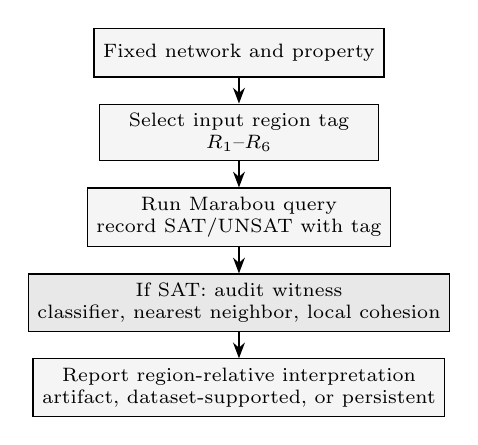
\begin{tikzpicture}[
  node distance=0.33cm,
  processbox/.style={draw, minimum height=0.62cm, minimum width=3.55cm, font=\scriptsize, align=center, fill=gray!8},
  audit/.style={draw, minimum height=0.62cm, minimum width=3.55cm, font=\scriptsize, align=center, fill=gray!18},
  arrow/.style={-{Stealth[length=2mm]}, thick},
  every node/.style={font=\scriptsize}
]
  \node[processbox] (task) {Fixed network and property};
  \node[processbox, below=of task] (region) {Select input region tag\\$R_1$--$R_6$};
  \node[processbox, below=of region] (solver) {Run Marabou query\\record SAT/UNSAT with tag};
  \node[audit, below=of solver] (auditnode) {If SAT: audit witness\\classifier, nearest neighbor, local cohesion};
  \node[processbox, below=of auditnode] (report) {Report region-relative interpretation\\artifact, dataset-supported, or persistent};

  \draw[arrow] (task) -- (region);
  \draw[arrow] (region) -- (solver);
  \draw[arrow] (solver) -- (auditnode);
  \draw[arrow] (auditnode) -- (report);
\end{tikzpicture}%
}
\caption{Region-tagged verification workflow. The method holds the network and property fixed, varies the encoded input region, records every Marabou verdict with its region tag, and audits recovered SAT witnesses before interpreting the result.}
\label{fig:workflow}
\end{figure}

We use TinyTaxiNet as the primary case study, an open-source surrogate for runway-perception tasks that has appeared in several TaxiNet-family verification studies. It maps $8 \times 16$ grayscale runway images to cross-track and heading error. Prior studies on TinyTaxiNet and related TaxiNet models adopt input abstractions tailored to their verification objectives, including per-image perturbation regions, activation-pattern-conditioned boxes, and generative front-end regions~\cite{wu2020,kadron2021,katz2022}. This paper instead holds the perception network and property family fixed while varying the encoded input region and auditing recovered witnesses.

The protocol treats the input region as an experimental variable. Doing so separates a preprocessing artifact from an 8D decoder-box result in P1, surfaces a dimensionality confound in P3, and isolates one empirically attested persistent failure mode in P4. In P3, reducing the query to a low-dimensional region raises verification by more than a factor of four; the matched random-subspace control shows that verification rate follows dimension, while local PCA exposes more CTE-side witnesses than random 8D regions at the same scale. In P4, the wrong-sign cross-track mode survives every tested region tightening and appears in the simulator dataset. The input region is therefore not just a solver setup detail in this case study; it determines the scope and evidentiary meaning of the verification result.

The study addresses three questions.
\begin{itemize}[nosep]
  \item \textbf{RQ1: Verdict sensitivity.} How do Marabou SAT/UNSAT verdicts change when the same network and related tracking properties are evaluated under different input-region constructions?
  \item \textbf{RQ2: Counterexample support.} Which SAT witnesses are supported by empirical behavior in the released simulator dataset, and which depend primarily on loose pixel-space over-approximation?
  \item \textbf{RQ3: Audit value.} Which diagnostics are needed to interpret SAT witnesses produced under learned or structured regions?
\end{itemize}

The work contributes no new solver algorithm; it contributes a verification protocol and reusable artifact for interpreting solver results when the input set is itself a modeling choice. We implement the region-relative workflow through three contributions.
\begin{enumerate}[nosep]
  \item \textbf{Region-tagged comparative protocol.} We define six region tags ranging from raw pixel boxes to latent, local, and linear-constraint regions, then verify the same property family under multiple regions. Each Marabou SAT/UNSAT verdict is paired with the input abstraction that produced it (Section~\ref{sec:claim_scope}), isolating changes caused by preprocessing invariants, learned support models, and structural filters. The released module makes this reporting discipline executable as a reusable template.
  \item \textbf{Postcondition-headroom diagnostic.} We give a closed-form input-Jacobian and saturating-perturbation diagnostic that separates input-region effects from specification-margin effects (Section~\ref{sec:p3_region_comparison}).
  \item \textbf{Witness-audit protocol.} We pair recovered SAT witnesses with classifier probability, nearest-real-image $L_2$ distance, and per-pair Lipschitz violation fraction (Sections~\ref{sec:plausibility_constrained},~\ref{sec:math_regions}). The audit distinguishes regional witnesses that remain far from the simulator image distribution from witnesses with empirical dataset support.
\end{enumerate}

A small MNIST ReLU MLP provides a transfer check for the broad-region versus encoded-support contrast (Section~\ref{sec:mnist}). Two external checks add independent data and solver coverage: VNN-COMP \texttt{mnist\_fc} tests the workflow on a VNN-COMP-distributed image classifier (Section~\ref{sec:external_transfer}), and LARD V2 tests broad-region witnesses and dataset-support audits on runway imagery independent of VerifyGAN (Section~\ref{sec:probe_lard}). The released artifact includes the reusable \texttt{region\_audit.py} module, TinyTaxiNet and MNIST instantiations, VNN-LIB baseline queries, experiment scripts, JSON results, and smoke tests; Section~\ref{sec:reproducibility} gives the module interface and runtime details.

The rest of the paper is organized as follows. Section~2 describes TinyTaxiNet and the released preprocessing pipeline. Sections~3 and~4 define the region tags and formal properties. Section~5 gives the main TinyTaxiNet probes and the MNIST, \texttt{mnist\_fc}, and LARD instantiations. Section~6 audits witnesses and stress-tests learned and math-encoded regions. Section~7 compares the protocol with related verification approaches, Sections~8--9 describe reproducibility and calibration checks, Section~10 discusses validity scope and future work, and Section~11 concludes.


% ============================================================
\section{System Under Verification and Preprocessing}

TinyTaxiNet is an open-source feedforward ReLU network distributed in the sisl/VerifyGAN repository~\cite{katz2022} as a compact surrogate for the Boeing TaxiNet perception network used in autonomous center-line tracking~\cite{kadron2021,pasareanu2023closedloop}. We use the repository's TinyTaxiNet artifacts, not the GAN-based verification method of Katz et al.~\cite{katz2022}. The network implements
\[
f: \mathbb{R}^{128} \to \mathbb{R}^{2}
\]
by mapping a flattened $8 \times 16$ grayscale runway image through three hidden layers (16, 8, 8 neurons with ReLU activation) to two outputs:
\begin{itemize}[nosep]
  \item $y_0$: cross-track error (CTE, meters from centerline)
  \item $y_1$: heading error (HE, degrees off alignment)
\end{itemize}

The network has 32 ReLU neurons ($16 + 8 + 8$) and 194 total variables in Marabou's encoding (inputs 0--127, outputs 192--193). Verification operates on the released post-preprocessed $128$-vectors described below.

\subsection{Data and Preprocessing}

We use the publicly available 10{,}000-image dataset and TinyTaxiNet weights from the sisl/VerifyGAN repository~\cite{katz2022}, produced by the SISL team.

\textbf{Preprocessing.} Each raw X-Plane screenshot is cropped, resized, converted to grayscale, downsampled to $8 \times 16$, then per-image mean-centered and clipped:
\begin{equation}
x \leftarrow \text{clip}\!\left(x - \overline{x} + 0.5,\; 0,\; 1\right)
\end{equation}
The flattened 128-vector is what gets saved to HDF5 and what we load for verification.

\textbf{Dataset:} 10{,}000 simulator-generated training images with labels (CTE, HE, DTP).

\textbf{Dataset and preprocessing checks.} All 10{,}000 images have pixel mean $= 0.5000$, confirming the mean-centering invariant. The \texttt{.nnet} file embeds no additional normalization, and we set \texttt{normalize=False} in Marabou to match the released inputs.

% ============================================================
\section{The Region Spectrum}
\label{sec:spectrum}

Marabou and other complete neural-network verifiers~\cite{wu2024marabou,katz2017reluplex,katz2019marabou} answer queries of the form $\forall x \in R . P(f(x))$, where $f$ is the network and $R$ is the encoded input region. Marabou returns SAT when a concrete counterexample exists in $R$ and UNSAT when the property holds for all inputs in $R$. The verdict is exact for the encoded formula; this section defines the six input-region tags used to state what that formula is.

\subsection{Verification regions}
\label{sec:claim_scope}

Every Marabou verdict in the paper is tagged with one of the six regions below. Formal definitions, Marabou encodings, and calibration details are in Appendix~\ref{app:construction_ref}.

\begin{itemize}[nosep]
  \item \textbf{$R_1$ (raw per-pixel box):} independent per-pixel bounds, either a subset envelope $R_1(S)$ or a per-image ball $R_1(x_0,\varepsilon)$.
  \item \textbf{$R_2$ ($R_1$ + mean invariant):} $R_1$ plus the preprocessing equality $\mathrm{mean}(x){=}0.5$.
  \item \textbf{$R_3$ (AE decoder-box, mean-constrained):} subset-specific ReLU autoencoder decoder composed with TinyTaxiNet over the train-only latent box.
  \item \textbf{$R_4$ (local-PCA per-image, mean-constrained):} top-$d{=}8$ same-state-neighbor principal directions around the query image, scaled by $\alpha\sigma$.
  \item \textbf{$R_5$ (label-conditioned box):} per-pixel $[\min,\max]$ over same-state neighbors of the anchor, intersected with clipping and the mean invariant.
  \item \textbf{$R_6$ (math-encoded, mean-constrained):} box-plus-mean intersected with linear-in-pixel image-structure filters: TV, Fourier high-frequency $L_1$, photometric residual, per-row mean, per-cell mean, or per-pair Lipschitz bounds.
\end{itemize}

Tags are parameterized by their calibration data, a subset $S$, an anchor $(x_0,\varepsilon)$, or both. Dataset-only observations are reported as empirical baselines, not solver regions, because they invoke no Marabou query and produce no SAT/UNSAT verdict.

\subsection{Dataset query domains}
\label{sec:input_regions}

Table~\ref{tab:regions} lists the dataset-level domains used to calibrate region bounds, latent boxes, PCA bases, and empirical filter thresholds.

\begin{table}[!h]
\centering
\sttttablefont
\setlength{\tabcolsep}{3pt}
\begin{tabular}{lllr}
\toprule
Subset & Definition & Used by & Images \\
\midrule
$C_\text{centered}$ & $|\text{CTE}| < 1.0$\,m & P1, P6 & 893 \\
$C_\text{left}$ & CTE $> 2.0$\,m & P4 & 4{,}128 \\
$C_\text{right}$ & CTE $< -2.0$\,m & P4 & 4{,}099 \\
$C_\text{off-center}$ & $|\text{CTE}| > 1.0$\,m & $R_3$ ($\mathrm{AE}_\text{off-center}$) & 9{,}107 \\
$L_\infty$ ball & $\|x - x_0\|_\infty \le \varepsilon$ & P2, P3 & per image \\
\bottomrule
\end{tabular}
\caption{Input subsets and query domains used to calibrate the region tags. Subset rows define dataset-level envelopes; the $L_\infty$ row is per-image.}
\label{tab:regions}
\end{table}

\subsection{Perturbation model and threshold rationale}
\label{sec:perturbation_model}

All $\varepsilon$ values in this paper are $L_\infty$ radii in post-preprocessed network-input space (after crop, resize, grayscale, $8{\times}16$ downsample, mean-center, clip); they characterize sensitivity of the network's learned function around real preprocessed inputs, not raw-camera or weather perturbation magnitudes. P2 and P3 use $\varepsilon \in \{0.02, 0.05, 0.10\}$. Same-state-neighbor calibration on the centered subset (closest other image with $|\Delta\text{CTE}|{\le}0.5$\,m, $|\Delta\text{HE}|{\le}5^\circ$): p10 $0.033$, p25 $0.060$, p50 $0.103$, p90 $0.189$. Random-pair $L_\infty$ median is $0.271$. Thus $\varepsilon{=}0.02$ is below the centered same-state p10, $\varepsilon{=}0.05$ between p10 and p25, $\varepsilon{=}0.10$ near the same-state median; all three lie well below the random-pair median.

Output thresholds follow Kadron et al.~\cite{kadron2021} where applicable: $|\text{CTE}|<10$\,m and $|\text{HE}|<90^\circ$ (P1/P3 output bounds; 10\,m is $\sim 22\%$ of the $\sim 46$\,m Grant County Runway~04 width, $90^\circ$ is complete loss of alignment); $|\Delta\text{CTE}|<1.0$\,m, $|\Delta\text{HE}|<5.0^\circ$ (P2 correctness). The remaining thresholds are case-study choices for TinyTaxiNet: P4 left/right at $|\text{CTE}|>2.0$\,m, P6 binary-search tolerance $0.01$.

% ============================================================
\section{Formal Specifications}

The baseline property set contains five Marabou encodings. Table~\ref{tab:specs} lists the exported baseline queries by property class.

\begin{itemize}[nosep]
  \item \textbf{Invariance / output-bound properties} (P1, P3): universal claims that for all inputs in a region, the output lies within an absolute box. Negation is a disjunction over bound violations.
  \item \textbf{Sign and relational properties} (P2, P4): universal claims about a relation between input/output or between output components. P2 relates output to a reference label; P4 relates output sign to input-region label.
  \item \textbf{Reachability / output-range property} (P6): an existential query about what outputs are reachable. P6 sweeps thresholds to find the tight reachable range for each output axis.
\end{itemize}

Invariance failures show that the network can exceed design bounds somewhere inside the encoded region; sign and relational failures show consistency violations inside that region; reachability results characterize the encoded output set itself.

\begin{center}
\begin{minipage}{\columnwidth}
\sttttablefont
\setlength{\tabcolsep}{2pt}
\begin{tabular}{p{0.18\columnwidth}p{0.58\columnwidth}r}
\toprule
Property & Encoded query & Queries \\
\midrule
P1-global & $x \in C_\text{centered}$; prove $|y_0|<10$ and $|y_1|<90$ with one sub-query per violated side & 4 \\
P1-patterned & P1 over each observed centered 32-bit activation pattern & 96 \\
P2 & $\|x-x_0\|_\infty \le 0.02$; prove $|y_0-y_0^*|<1.0$ and $|y_1-y_1^*|<5.0$ & 160 \\
P3 & $\|x-x_0\|_\infty \le \varepsilon$; prove the P1 output envelope around sampled anchors & 160 \\
P4 & $x \in C_\text{left/right}$; prove the CTE output sign matches the offset side & 2 \\
P6 & $x \in C_\text{centered}$; binary-search tight reachable intervals for $y_0$ and $y_1$ & 52 \\
\bottomrule
\end{tabular}
\refstepcounter{table}\label{tab:specs}
\smallskip
\noindent\textbf{Table~\thetable}\quad Baseline exported formal queries by property class. Strict inequalities are negated using Marabou's non-strict bound API. P2/P3 use 20 evenly spaced baseline images; P6 uses binary search with tolerance $0.01$.
\end{minipage}
\end{center}

\textbf{Property use.} P1, P3, and P4 are evaluated under multiple region constructions. P2 evaluates local correctness under a small $L_\infty$ ball, and P6 characterizes reachable output bounds over the centered box. P1-patterned partitions $C_\text{centered}$ by the 32-bit activation pattern across all hidden layers and verifies each observed pattern; only the 24 centered-image patterns are visited, the others have no empirical evidence of occurrence. Property numbering follows the released artifact identifiers; P5 was superseded during revision and is not part of the baseline set.

% ============================================================
\section{Three Probes}
\label{sec:probes}
\label{sec:results}

The primary results are P1, P3, and P4 (Table~\ref{tab:results}). P1 separates a preprocessing artifact from an 8D decoder-box claim, P3 measures sensitivity to region dimension and orientation, and P4 tracks a failure mode that survives every tested region tightening. Section~\ref{sec:probe_mnist} applies the same protocol to MNIST as a transfer check.

\begin{table*}[!t]
\centering
\sttttablefont
\setlength{\tabcolsep}{5pt}
\begin{tabular}{l c >{\raggedright\arraybackslash}p{4.4cm} >{\raggedright\arraybackslash}p{1.8cm}}
\toprule
Property & Region & Result & Failure axis / note \\
\midrule
P1-global       & $R_1$         & Violated; three of four sub-queries SAT & CTE both; HE lower \\
P1-patterned    & $R_1$         & 16/24 patterns proved & CTE in 8 patterns \\
P1a, P1b        & $R_3$         & UNSAT in 8D decoder-box; random 8D affine also UNSAT (dimensionality) & none in-region \\
P2 ($\varepsilon{=}0.02$) & $R_1$ & 0/893 robust on centered subset (69\% wrong, 31\% fragile) & Both \\
P3 & $R_2$, $R_4$ & $R_2$: 186/893; $R_4(1\sigma)$: 847/893; rand. 8D$(1\sigma)$: 893/893 & Dim.; CTE SATs \\
P4 base         & $R_1$         & SAT, CTE${=}0$ (boundary) & wrong-sign \\
P4 sweep        & $R_3$         & SAT at $|\text{CTE}|{\ge}3$ & wrong-sign (1.7\% emp.) \\
P6              & $R_1$         & CTE $[-24.3, 23.3]$ & per-axis env. \\
P1/P4 (math)    & $R_6$         & SAT at all main calibrations; most stored witnesses rejected by both classifier audits & requires witness audit \\
\bottomrule
\end{tabular}
\caption{Summary of region-tagged TinyTaxiNet verification results. The Region column uses the tags defined in Section~\ref{sec:claim_scope}; detailed P3 status counts appear in Figure~\ref{fig:p3_status_bars}. The random-control entry is the matched 8D control at $1\sigma$; at $2\sigma$ and $3\sigma$ the control also verifies more often than local PCA but is not witness-free.}
\label{tab:results}
\end{table*}

\begin{figure*}[t]
\centering
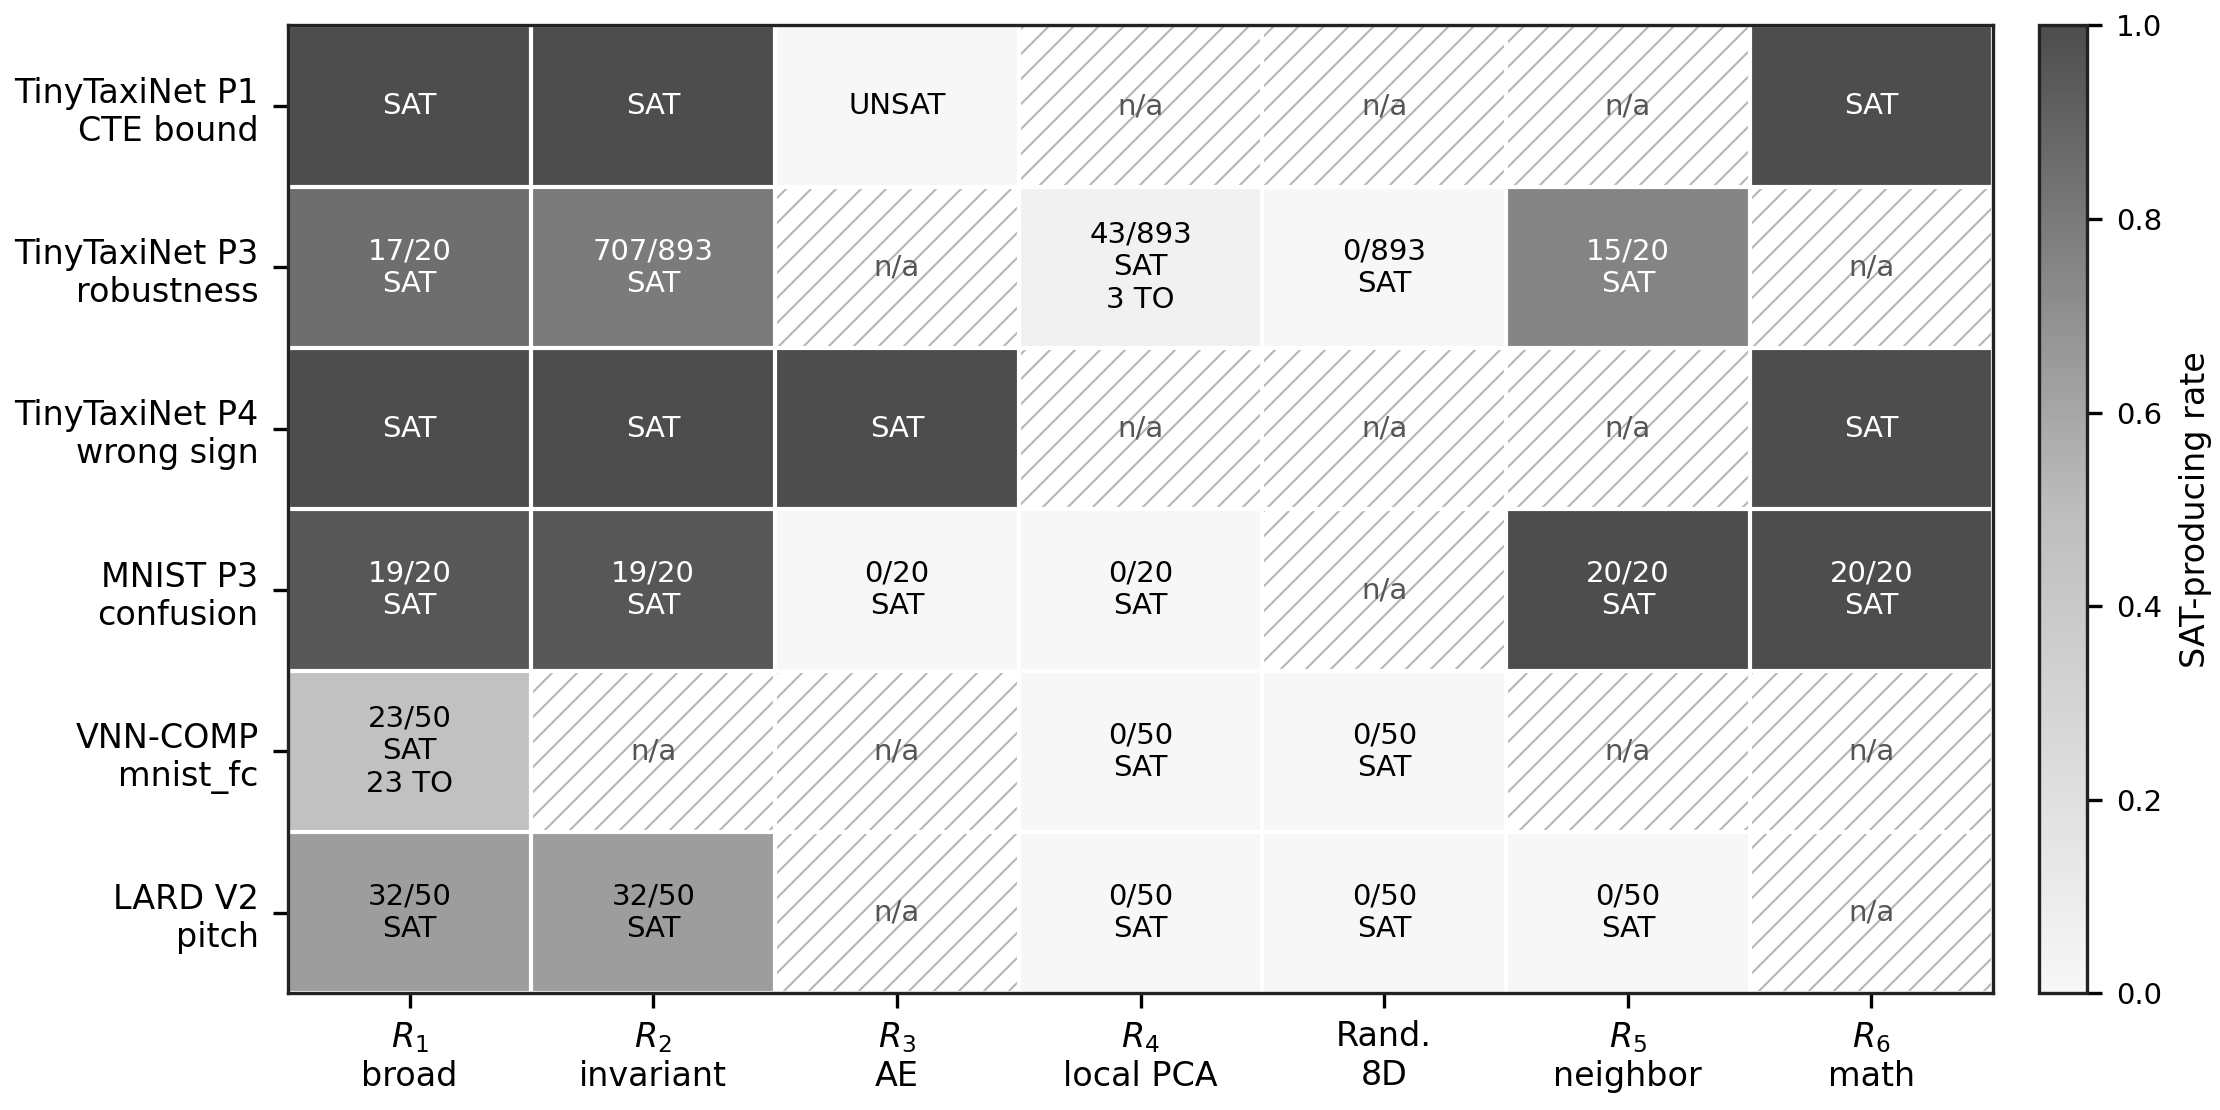
\includegraphics[width=\textwidth]{region_transition_heatmap.png}
\caption{Region-tagged verdict changes across the main instantiations. Cell color gives the SAT-producing rate for the indicated property/region pair; hatched cells are not part of that experiment. Labels report the exact counts used in the paper, with ``TO'' denoting timeouts. Because rows use different sample sizes and timeout profiles, colors are descriptive rather than equal-denominator statistical comparisons; the printed denominators are the authoritative values. The TinyTaxiNet P3 row uses expanded all-893 counts for $R_2$, $R_4$, and the matched random 8D control where available; the $R_1$ and $R_5$ cells remain the original 20-anchor diagnostic counts. The \texttt{mnist\_fc} row shows the pre-rerun broad-ball counts; Table~\ref{tab:external_instantiations} reports the post-rerun counts. P1 $R_3$ has the matched random-affine control reported in Section~\ref{sec:probe_p1}; the compact-MNIST learned-region cells are encoded-region verdicts without matched random-8D controls. The figure highlights the transition patterns: preprocessing removes P1d, low-dimensional regions drive the P3 and external witness removals, and the TinyTaxiNet P4 wrong-sign mode persists across tested tightenings.}
\label{fig:region_transition_heatmap}
\end{figure*}

\subsection{P1: box artifact and AE-region result}
\label{sec:probe_p1}
\label{sec:p1_results}

P1-global evaluates whether every input in the centered per-pixel box remains inside the Kadron-style tracking envelope. Over the raw region $R_1$, the property is \textbf{violated}: three of four sub-queries return SAT.
\begin{itemize}[nosep]
  \item P1a (CTE $\ge 10$): SAT. Witness: CTE $= 10.0$, HE $= -52.5^\circ$.
  \item P1b (CTE $\le -10$): SAT. Witness: CTE $= -10.0$, HE $= 15.0^\circ$.
  \item P1c (HE $\ge 90$): \textbf{UNSAT}. No centered input produces HE $\ge 90^\circ$.
  \item P1d (HE $\le -90$): SAT. Witness: CTE $= 18.5$, HE $= -90.0^\circ$.
\end{itemize}

P1-patterned tightens the same centered query by partitioning it according to the 24 observed Prophecy/Kadron-style activation patterns~\cite{prophecy2019,kadron2021}; each pattern is the complete 32-bit sign vector across the hidden ReLUs. The partitioned run verifies \textbf{16/24 patterns} ($66.7\%$ of observed patterns; 378/893 centered images, $42.3\%$ image coverage). The remaining 8 patterns fail exclusively on CTE, and the four largest failed patterns contain $\sim 86\%$ of images in violated regions. Sparse execution paths become provable, but the patterns covering most centered data remain too broad to establish the global P1 bound.

\textbf{Mean-constrained follow-up:} Enforcing $\text{mean}(x) = 0.5$ separates the heading-side artifact from the lateral-side failures. P1d flips from SAT to UNSAT, so the HE $\le -90^\circ$ witness was enabled by a missing preprocessing invariant. P1a and P1b remain SAT, so the CTE-side failures are not removed by mean centering alone.

\textbf{P1d disappears under $R_2$; P1a/P1b persist until $R_3$.} P1d is SAT only under $R_1$: no image in the full 10{,}000-image dataset has $|\text{HE}_\text{err}| > 90^\circ$ (empirical maximum $62.6^\circ$), and the query becomes UNSAT once the mean invariant is enforced in $R_2$ and $R_3$ (Section~\ref{sec:plausibility_constrained}). P1a and P1b remain SAT under $R_1$ and $R_2$ and flip to UNSAT under the 8D AE decoder-box region $R_3$, but the centered empirical CTE-error maximum is only $4.64$\,m, well below the $10$\,m threshold; the 23 full-dataset images exceeding $10$\,m are all off-center. The lateral SAT witnesses are not directly observed centered-state failures. A matched-dimension control tests the source of the flip: deterministic zero-mean orthonormal random 8D affine regions, calibrated to the centered subset's projection box as $x = \mu + V^\top z$ with $0\le x\le1$, flip both P1a and P1b to UNSAT across three seeds; the corresponding PCA 8D affine region also flips both queries. The control regions are non-degenerate: a reproducible corner/random validation search reaches CTE magnitudes of $7.9$\,m for PCA and $2.4$--$3.9$\,m for random, while the exact Marabou queries prove the $10$\,m bound is not reachable in those regions. The matched control assigns the P1a/P1b $R_3$ flip to the 8D restriction rather than decoder-specific support; PCA reaches closer to the bound than random, the same data-alignment signal quantified for P3.


\subsection{P3: region-dependent robustness}
\label{sec:probe_p3}
\label{sec:p3_results}

P3 asks whether predictions remain inside the broad $\pm 10$\,m, $\pm 90^\circ$ output envelope under local perturbation. We evaluate matched centered anchors under unconstrained $L_\infty$ balls, mean-constrained and clipped $L_\infty$ balls, and local-PCA regions calibrated to same-state image variation. The full-centered mean$+$clip run verifies 892/893 images at $\varepsilon=0.02$, 186/893 at $\varepsilon=0.05$, and 0/893 at $\varepsilon=0.10$.

P3 verifies 3--4/20 at $\varepsilon = 0.05$ while P2 verifies 0/20 at the smaller $\varepsilon = 0.02$ because P2 tests a 1\,m correctness band and P3 tests a 10\,m output envelope. All P3 failures under these $L_\infty$ balls are CTE-driven. Under the mean-constrained ball, 707/893 centered states at $\varepsilon = 0.05$ and all 893 at $\varepsilon = 0.10$ admit a perturbation that pushes lateral offset beyond the $\pm 10$\,m envelope.


\subsubsection{\texorpdfstring{Region Comparison: pixel $L_\infty$ vs.\ label-conditioned box vs.\ local PCA}{Region Comparison: pixel L-infinity vs. label-conditioned box vs. local PCA}}
\label{sec:p3_region_comparison}

\textbf{Does per-pixel independence drive the fragility?} The mean-constrained $L_\infty$ ball still permits arbitrary independent per-pixel deviations. To test how much of P3's CTE fragility requires those directions, we re-verify under the label-conditioned box and local-PCA regions, both with $\text{mean}(x) = 0.5$ and clipping enforced. Each local-PCA anchor carries its own neighbor set and PCA basis. The expanded run covers all 893 centered images for $\alpha{=}1\sigma$ and $2\sigma$, and a deterministic 200-anchor subset for the more expensive $\alpha{=}3\sigma$; the selection rule, region parameters, PCA dimension, and 300\,s per-query timeout are identical across sample sizes.

\begin{figure*}[htbp]
\centering
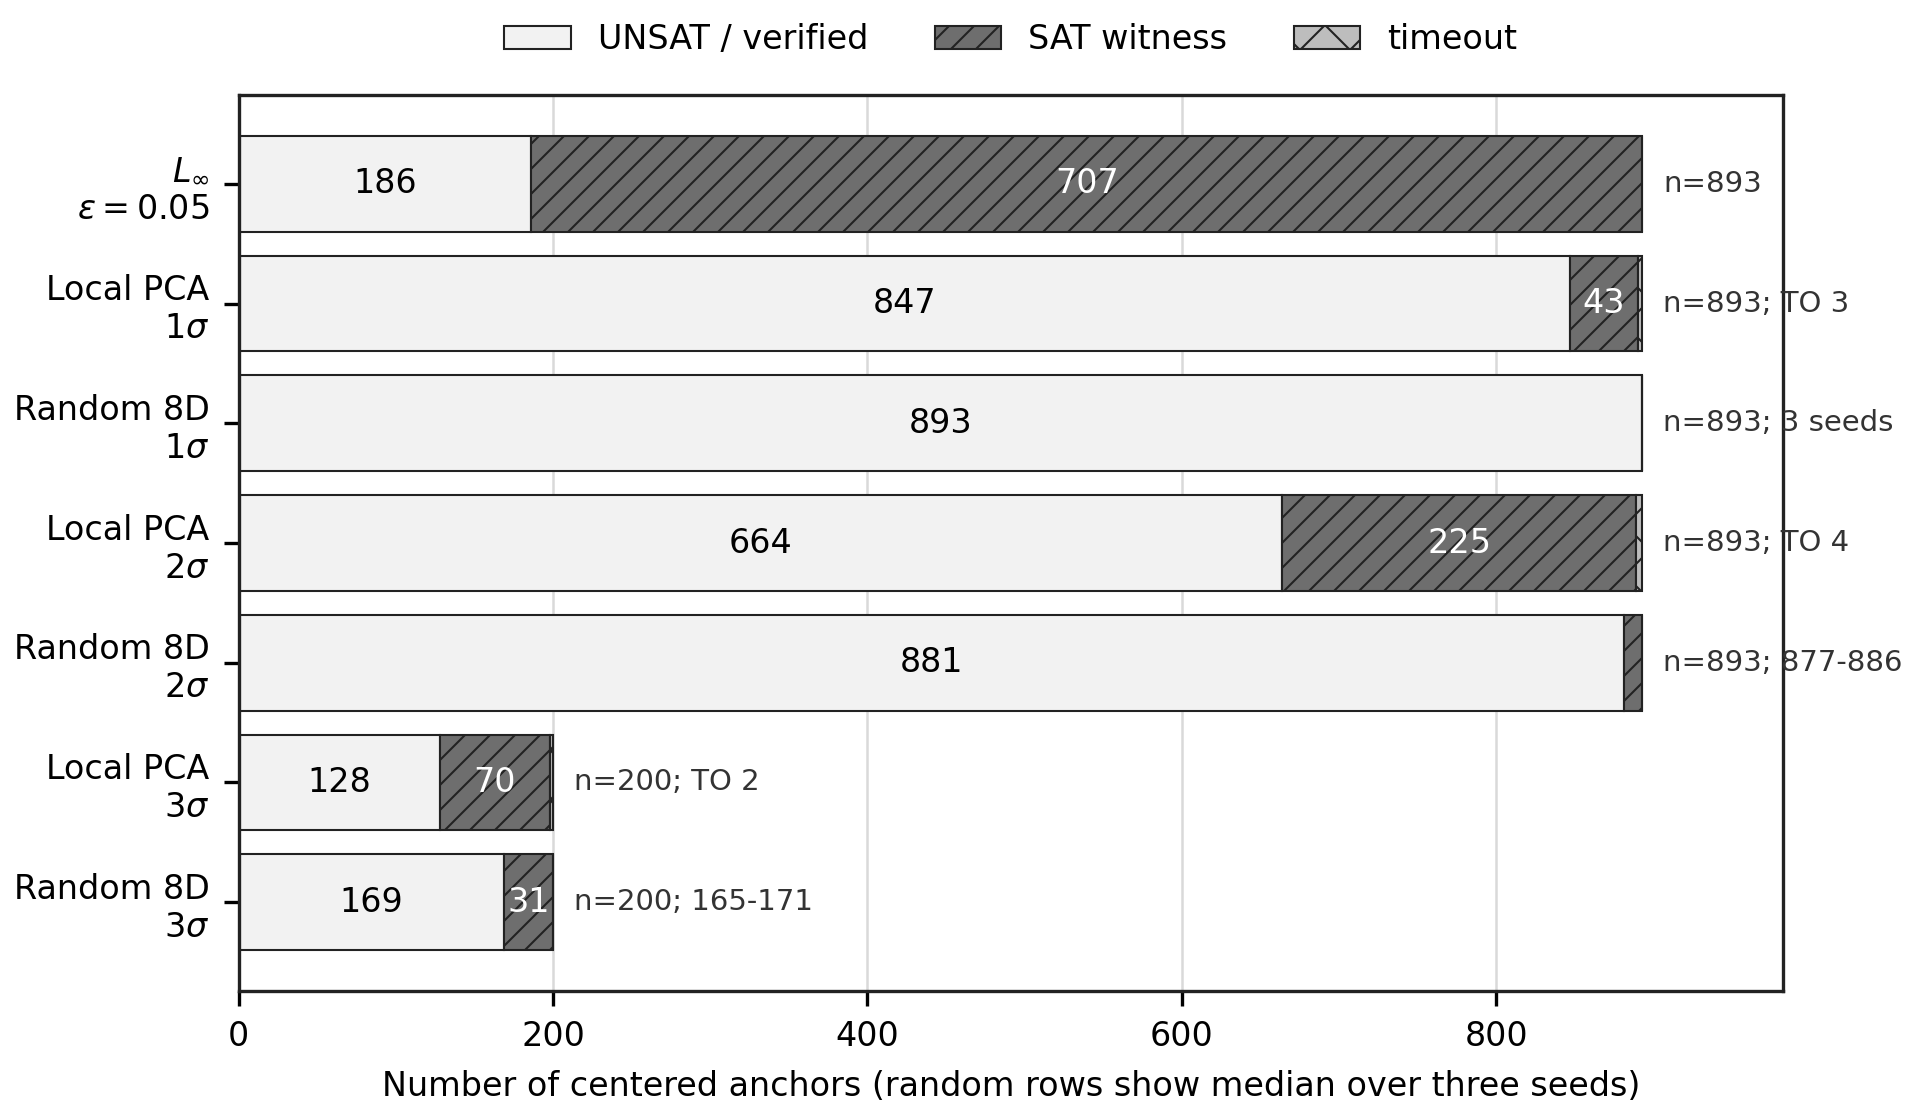
\includegraphics[width=0.82\textwidth]{p3_status_bars.png}
\caption{Expanded P3 status counts generated from the released artifacts. The $L_\infty$ row is the full centered mean$+$clip run at $\varepsilon=0.05$; local PCA and matched random 8D controls at $1\sigma$ and $2\sigma$ cover all 893 centered images, while the $3\sigma$ rows use the deterministic 200-anchor subset. Random rows report the median count over three seeds with the verified-count range printed at right when nonzero. At $1\sigma$, the random controls have zero SAT witnesses, while local PCA has 43 CTE-side SAT witnesses. Timeouts are reported separately and are not counted as verified.}
\label{fig:p3_status_bars}
\end{figure*}

Verification rates increase from 186/893 (20.8\%) under the mean-constrained $L_\infty$ ball to 847/893 (94.8\%) under local PCA at $\alpha = 1\sigma$ and 664/893 (74.4\%) at $\alpha = 2\sigma$ on all 893 centered images, confirming at full scale the region-dimension contrast first seen on the 20-anchor sample (4/20 to 20/20 and 17/20). Timeouts are reported separately in the figure caption and are not counted as verified. The rate falls monotonically as the local-PCA region loosens (94.8\%, 74.4\%, and 64.0\% at $3\sigma$ on the deterministic 200-anchor subset), and the expansion surfaces region witnesses the small sample missed: 43 anchors are SAT at $1\sigma$ and 225 at $2\sigma$, so local PCA tightens the search space but does not eliminate P3 fragility across the full set. The label-conditioned per-pixel box is barely tighter than the same-radius $L_\infty$ ball (5/20 vs.\ 4/20), because the solver still chooses independent excursions across all 128 pixels. This $R_5$/$R_4$ contrast is the mechanistic point: per-pixel independence remains loose even when the per-pixel bounds are calibrated from same-state neighbors, while the local affine region removes those independent directions. The witnesses are overwhelmingly CTE-driven: at $1\sigma$ every region witness is CTE-side, with no HE violation among the 893 anchors, while looser regions admit a few HE-side witnesses (8 of 893 at $2\sigma$, 20 of 200 at $3\sigma$).

\textbf{Is the rate gain a dimension effect?} The verification-rate gain could come from reducing the verifier to an 8D region rather than from the specific data-conditioned PCA directions. We separate the two with a matched control that swaps the PCA basis for deterministic zero-mean orthonormal random 8D directions (three seeds), reusing each anchor's local-PCA per-direction scale $\sigma_j$, the mean invariant, clipping, thresholds, and solver settings, so only the orientation changes; the bases are orthonormal and zero-mean to $10^{-15}$. Random subspaces verify at least as often as local PCA at every scale: 893/893 at $1\sigma$, 881/893 (median; range 877--886) at $2\sigma$, and 169/200 (165--171) at $3\sigma$, versus 847/893, 664/893, and 128/200 for local PCA, with no timeouts in the control. The verification-rate improvement over the mean-constrained $L_\infty$ ball is thus a low-dimensional-region effect. Local PCA is the stronger falsification region: its data-aligned axes recover CTE-side witnesses a random subspace misses (43 vs.\ 0 SAT at $1\sigma$; 225 vs.\ a median 12 SAT at $2\sigma$), while its verification rate is lower than the random control. Figure~\ref{fig:p3_frontier} plots the verification/support trade: the random 8D subspace attains the highest verification rate but captures little same-state variation, whereas local PCA pairs high verification at small $d$ with a defined support metric. The two quantities are reported separately through region tags and witness audits.

\begin{figure}[t]
\centering
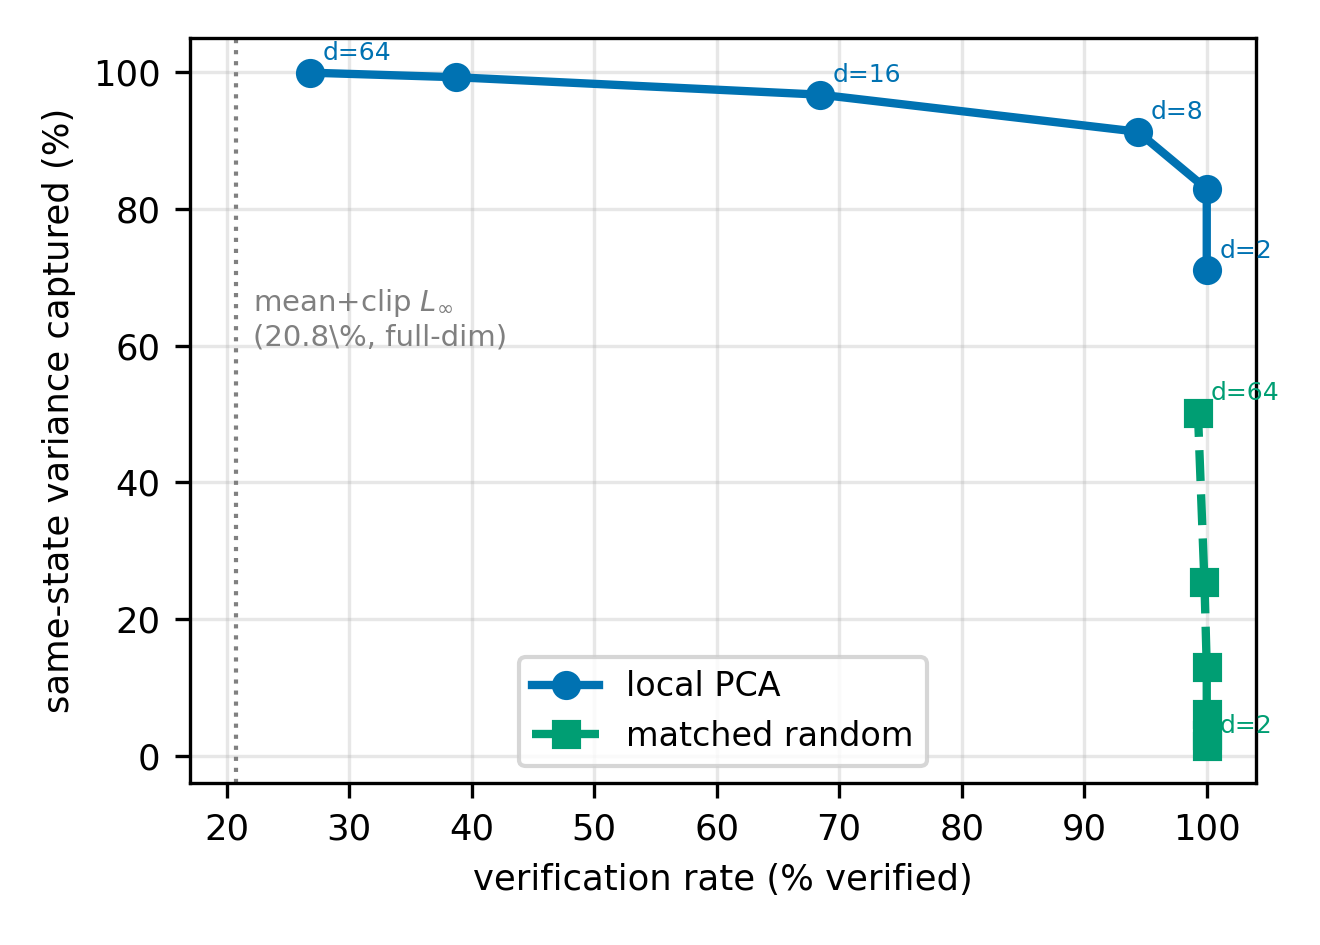
\includegraphics[width=0.82\linewidth]{p3_coverage_verification_frontier_figure.png}
\caption{Verification rate versus same-state variance captured by the subspace (TinyTaxiNet P3, $\alpha{=}1\sigma$). Random subspaces verify more often but capture little data variation; local PCA captures more variation and therefore finds CTE-side witnesses as $d$ increases. The full-dimensional $L_\infty$ point has no comparable low-dimensional membership metric.}
\label{fig:p3_frontier}
\end{figure}

\textbf{Where does direction start to matter? A dimension sweep.} Fixing $\alpha{=}1\sigma$ and sweeping the subspace dimension $d\in\{2,4,8,16,32,64\}$ separates dimensionality from orientation across scales on the $694$ centered anchors with at least $d{+}1$ same-state neighbours at $d{=}64$ (Fig.~\ref{fig:dimsweep}). At small $d$ the two bases agree: both verify $100\%$ at $d{\le}4$, and $94.4\%$ (PCA) versus $100\%$ (random) at $d{=}8$, so at the operating point the rate gain is a dimension effect. As $d$ grows the curves diverge sharply: local-PCA verification collapses to $68.4\%$, $38.8\%$, and $26.8\%$ at $d{=}16,32,64$ (with $18$, $33$, and $26$ timeouts, reported separately and not counted as verified), while the matched random subspace stays at $100\%$, $99.8\%$, and $99.3\%$. Data-conditioned directions therefore begin to matter at $d\gtrsim16$: a larger PCA subspace captures the data variation that reaches the CTE bound, whereas a random subspace at the same $\sigma$ scale spends its dimensions on generic directions and stays far from the bound. Splitting the four P3 sub-queries by axis over the $200$-anchor candidate subset (the $159$ anchors with at least $65$ same-state neighbours, scored at every $d$) shows the growth is cross-track-driven: the count of anchors with a CTE counterexample climbs with dimension ($0, 0, 9, 43, 95, 107$ at $d{=}2,4,8,16,32,64$), while heading-side counterexamples appear only at $d\ge32$ and stay rare ($2$ then $7$ anchors). The data-aligned directions thus reach the $\pm10$\,m CTE envelope well before the $\pm90^\circ$ HE envelope. The external LARD replication (queries $\sim1.6$\,s each) shows both bases removing all broad witnesses at every $d\le64$, consistent with witnesses lying outside the data-variance envelope at matched scale.

\begin{figure}[t]
\centering
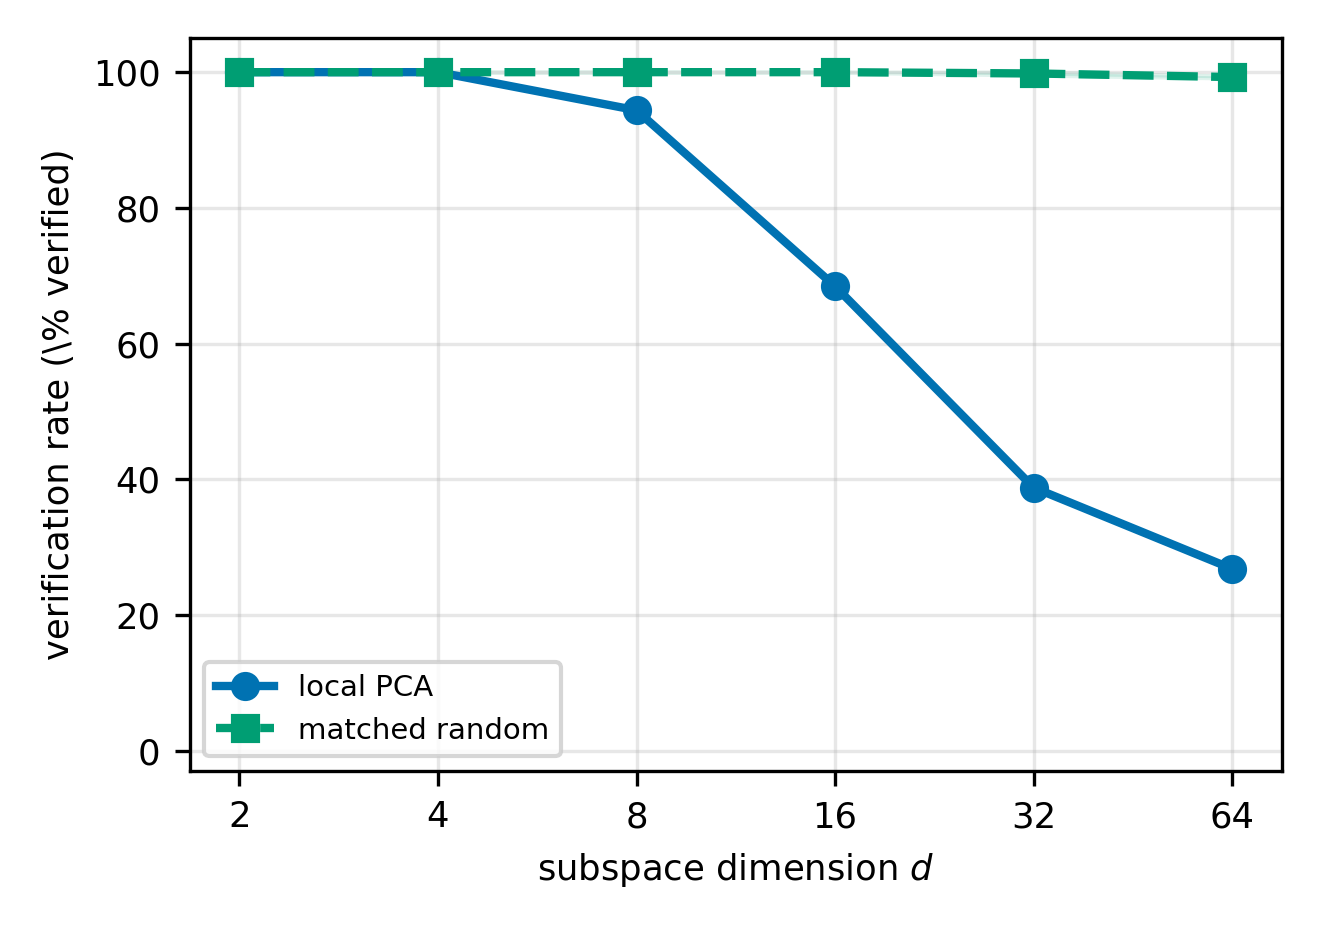
\includegraphics[width=0.82\linewidth]{p3_dimension_sweep.png}
\caption{P3 verification rate versus subspace dimension $d$ at $\alpha{=}1\sigma$ (TinyTaxiNet, $694$ anchors). Local PCA and the matched random subspace agree at small $d$ but diverge at $d\gtrsim16$: PCA verification collapses (its data-aligned directions reach the CTE bound) while the random subspace stays near $100\%$. Timeouts are reported separately and not counted as verified.}
\label{fig:dimsweep}
\end{figure}

\textbf{A cheap subspace attack does not substitute for the solver.} On the identical local-PCA regions, a multi-restart corner-jump/PGD attack ($30$ restarts and $50$ iterations per objective, $0.10$\,s per region, valid-pixel witnesses only) finds none of the joined Marabou-SAT witnesses at $d{=}8$: $0$ attack witnesses against $33$, $225$, and $70$ joined SAT verdicts at $\alpha{=}1,2,3\sigma$, with $0$ attack-only witnesses and $622$, $664$, and $128$ UNSAT certificates the attack cannot provide. The $\alpha{=}1\sigma$ attack records cover 657 of the 893 anchors, including 33 of the 43 Marabou SAT anchors reported above; the remaining 10 SAT anchors are outside the attack-record join, not contradictory verdicts. The $\alpha{=}2\sigma$ and $3\sigma$ joins cover the full local-PCA runs at those scales. The attack's best objective falls short of the P3 bound by a median of $6.4$ at $d{=}8$; on a representative SAT anchor a $500$-restart stress run reaches $\mathrm{CTE}=-1.4$ against Marabou's feasible $-10$. Formal solving is decisive on these regions: it recovers SAT witnesses the attack misses and certifies UNSAT where attack failure is inconclusive.

The local-PCA witnesses have mixed audit support: across the 14 CTE-side witnesses recovered at $\alpha=2\sigma$ and $3\sigma$ on the 20-anchor sample, median classifier probability is $0.07$ (real images: median $0.95$), median nearest-real-image $L_2$ distance is $0.80$, and 4/14 score above probability $0.9$.

\textbf{Is CTE dominance an input-region effect or a specification effect?} Closed-form input Jacobians show that the CTE-dominated failure pattern is not caused by lower HE sensitivity. On all 893 centered images, the exact local Jacobian $J(x)=\partial(\mathrm{CTE},\mathrm{HE})/\partial x$ (finite-difference relative error below $10^{-11}$) gives median norms $\|J_{\mathrm{HE}}\|_1=649$ vs.\ $\|J_{\mathrm{CTE}}\|_1=259$ and $\|J_{\mathrm{HE}}\|_\infty=41.7$ vs.\ $\|J_{\mathrm{CTE}}\|_\infty=8.5$. The network is therefore $2.5$--$4.9\times$ more pixel-sensitive on HE than on CTE in these norms. In first-order margin terms, the observed asymmetry is explained by postcondition headroom: median centered prediction is $|y_0|=1.68$\,m vs.\ $|y_1|=14.7^\circ$, leaving median headroom of $8.32$\,m and $75.3^\circ$. The median first-order pixel radius that saturates each bound is $\varepsilon_{\mathrm{CTE}}^{\mathrm{sat}}=0.0345$ vs.\ $\varepsilon_{\mathrm{HE}}^{\mathrm{sat}}=0.121$, so the tested $\varepsilon \in \{0.02,0.05,0.10\}$ span the CTE radius but remain at or below the median HE radius.

\textbf{Controlled postcondition sweep.} Holding the region fixed (mean-constrained $L_\infty$ ball, $\varepsilon{=}0.05$) and varying only the postcondition bound confirms the headroom explanation. The first-order violation fraction crosses $50\%$ at a CTE bound of $15$\,m and an HE bound of $50^\circ$, close to the corresponding headroom predictions of $14.7$\,m and $47.2^\circ$. Setting the HE bound to $35.4^\circ$, which equalizes the median saturating radius with the CTE $10$\,m bound, removes the original CTE-dominated pattern: at $\varepsilon{=}0.0345$ the two axes violate at matched rates ($50.2\%$ CTE, $50.1\%$ HE), and at $\varepsilon{=}0.05$ the exact Marabou run on the 20-image P3 sample changes from CTE $16/20$ vs.\ HE $0/20$ at the original bounds to CTE $16/20$ vs.\ HE $15/20$ under the equalized HE bound.

\subsection{P4: directional failure across regions}
\label{sec:probe_p4}
\label{sec:p4_results}

P4 tests directional sign consistency on the left and right offset domains. Both $C_\text{left}$ and $C_\text{right}$ return \textbf{SAT} under the raw per-pixel box. The initial baseline witnesses lie at the programmatic boundary of the strict sign inequality (CTE $=0.0$\,m), establishing feasibility without characterizing failure severity. The empirical baseline shows that the same qualitative failure mode is already present on real dataset images: 92/4{,}128 left images (2.2\%) and 50/4{,}099 right images (1.2\%) produce wrong-sign CTE.

\textbf{Mean-constrained and structured follow-ups:} Enforcing $\text{mean}(x) = 0.5$ preserves the SAT verdict. The released threshold sweep shows that P4-left wrong-sign witnesses survive under $R_2$ at $\text{CTE} \le -20$\,m; the same threshold remains SAT when $R_2$ is intersected with the tested math filters, including TV~$\le 2$ and Fourier~$\le 0.62$, both below the empirical centered-subset minima. The $C_\text{right}$ base query is similarly SAT. Empirical wrong-sign magnitudes reach $-3.51$\,m on the left-offset subset and $+3.28$\,m on the right-offset subset (Section~\ref{sec:plausibility_constrained}).

\textbf{Empirical and regional evidence.} ``Offset'' here means $|\text{CTE}|>2$\,m ($8{,}227$ images). The wrong-sign rate varies with distance from the centerline: 143/432 images (33.1\%) in the near-center band $0.5<|\mathrm{CTE}|<1$\,m are wrong-sign, compared with 142/8{,}227 (1.7\%) in the offset subset used for P4 and 41/5{,}490 (0.75\%) beyond $|\mathrm{CTE}|>5$\,m. The maximum wrong-sign magnitudes in those bands are 3.89\,m, 3.51\,m, and 2.28\,m, respectively. Within the offset subset, the wrong-sign mode is concentrated near the decision boundary: the rate falls from $6.3\%$ at $|\mathrm{CTE}|\in[2,3)$\,m to $0.5\%$ at $[5,8)$\,m, $58\%$ of wrong-sign cases have $|\text{predicted CTE}|<1$\,m, and $12\%$ have $|\text{predicted CTE}|>2$\,m. The wrong-sign images cluster more tightly than random offset images (mean pairwise $L_2$ $0.97$ vs.\ $1.13$), each one's nearest real neighbour is same-side, and left-side confusions outnumber right ($92$ vs.\ $50$). This characterizes P4 as a localized small-offset, near-boundary regression mode with dataset support. Wilson intervals on these rates treat the released $10{,}000$-image dataset as a sample from the simulator's image-generating process; on the dataset itself the rates are exact counts.

The P4 evidence has three layers. The released simulator images provide direct dataset support: 142/8{,}227 offset images exhibit wrong-sign CTE, with magnitudes up to 3.51\,m. The AE-composed P4 sweep shows the same sign failure persists inside subset-specific decoder-box regions, with witnesses up to $-3.42$\,m and $+3.00$\,m. The math-region threshold sweep shows that linear image-structure filters do not remove P4-left: $\mathrm{CTE}\le-20$\,m remains feasible under every tested math region, so those witnesses are paired with the downstream support audit in Section~\ref{sec:math_regions}.

\textbf{Contrast with Boeing TaxiNet.} Pasareanu et al.~\cite{pasareanu2023closedloop} report \emph{zero} blatant left/right confusion on the experimental Boeing TaxiNet (24-layer CNN, ELU activations): in their confusion matrix, no ground-truth ``far left'' CTE label is ever predicted ``right'' or vice versa.

\subsection{Supporting diagnostics}
\label{sec:supporting_diagnostics}
\label{sec:p2_supporting}
\label{sec:p6_results}

\textbf{P2 (local correctness).} P2 tests strict local functional correctness under an $L_\infty$ ball of radius $\varepsilon{=}0.02$ with a $1.0$\,m CTE band. It verifies $0/893$ centered images under both $R_1$ and $R_2$, and remains $0/893$ when the CTE band is relaxed to $1.5$\,m. On the full centered subset, $615/893$ images ($68.9\%$) are nominally wrong at $x_0$ and $278/893$ ($31.1\%$) are nominally correct but fragile inside the ball. The 20-image sample tracks the P3 20-anchor verification rates but has a different P2 wrong/fragile split ($9/20$ vs.\ $11/20$), so P2 is reported as a full-subset diagnostic.

\textbf{P6 (box-envelope width).} P6 resolves the absolute output envelope over $C_\text{centered}$ by binary search (52 queries, tolerance $0.01$). The certified bounds are $\mathrm{CTE} \in [-24.33, 23.30]$\,m and $\mathrm{HE} \in [-90.10, 84.07]^\circ$ against empirical centered-prediction ranges $[-4.95, 4.86]$\,m and $[-32.0, 33.3]^\circ$. These 4.86$\times$ and 2.67$\times$ over-approximation ratios measure the size of the box-abstraction headroom that P1d exploits.

\subsection{Probe synthesis}
\label{sec:probe_synthesis}

The three TinyTaxiNet probes produce transition patterns across regions. A verdict that disappears when the mean invariant is enforced points to a preprocessing-boundary issue; a verdict that disappears under a learned decoder-box and also under a matched random 8D region points to dimensionality rather than the support model, as in P1a/P1b under $R_3$; a high verification rate that also appears under random 8D regions points to dimensionality, with the PCA/random divergence at $d\gtrsim16$ marking where orientation begins to matter; and a verdict that survives every tested tightening while also appearing in simulator data points to behavior that input-side region tightening alone does not explain.

\textbf{Using the workflow on a new witness.} Given a SAT witness $W$ recovered under a broad region $R_1$, the workflow reruns the same query under tagged tighter regions (mean invariant, decoder box, local PCA, and a matched random 8D control at the same scale), audits $W$ with the three dataset-support signals, and records the transition pattern. A witness that disappears under a tighter region and scores off-manifold is a box-abstraction artifact, as in P1d after adding the mean invariant. A witness removed by both a learned 8D region and a matched random 8D region at the same scale is a dimensionality-sensitive result, as in P1a/P1b under $R_3$ and P3 at $d{=}8$. A witness that survives the tighter regions and occurs in the dataset is a dataset-supported finding, as in the localized P4 wrong-sign mode. Timed-out reruns remain unresolved. The controlled-oracle calibration exercises the same decision process on a known-truth semantic failure.

\subsection{Transfer check on MNIST}
\label{sec:probe_mnist}
\label{sec:mnist}

We apply the same three-probe structure to a compact MNIST ReLU MLP ($784 \to 32 \to 16 \to 10$, 48 hidden ReLUs, test accuracy $96.94\%$) as a transfer check: one network, 20 anchors, three class-confusion properties, and the same three audit signals. The six region tags are recalibrated to MNIST: per-image or per-class pixel boxes, a class-conditioned total-mass band, class-specific ReLU autoencoder boxes, local PCA over same-class neighbors, nearest-neighbor same-class boxes, and per-class total-variation bounds. MNIST has no exact preprocessing equality comparable to TinyTaxiNet's mean invariant, so its $R_2$ is a statistical band. The learned regions are coarser than in TinyTaxiNet: class-AE reconstruction $L_\infty$ median is $0.53$--$0.85$ per class, and the top-8 local-PCA directions capture $75\%$ of same-class-neighbor variance on average, versus $92\%$ on TinyTaxiNet.

Table~\ref{tab:mnist_verdicts} reports the MNIST verdict rates. Broad pixel regions admit class-confusion witnesses, while the learned AE and local-PCA regions remain UNSAT over their encoded supports. No matched random-8D control is reported for this compact MNIST MLP, so the $R_3$/$R_4$ UNSAT columns are encoded-region verdicts rather than evidence that learned orientation drives the flip.

\begin{table*}[htbp]
\centering
\sttttablefont
\setlength{\tabcolsep}{4pt}
\begin{tabular}{p{0.30\textwidth}p{0.34\textwidth}p{0.12\textwidth}p{0.12\textwidth}}
\toprule
Region & P3 SAT & P1 SAT & P4 SAT \\
\midrule
$R_1(x_0,\varepsilon)$ per-image $L_\infty$ ball & 2/20, 19/20, 20/20 at $\varepsilon=.01,.05,.10$ & 10/10 & 10/10 \\
$R_2(x_0,\varepsilon)$ ball + total-mass band & 2/20, 19/20, 20/20 at $\varepsilon=.01,.05,.10$ & 10/10 & 10/10 \\
$R_3$ class-AE decoder-box composition & \textbf{0/20} & \textbf{0/10} & \textbf{0/10} \\
$R_4$ local PCA, $\alpha = 2\sigma$ & \textbf{0/20} & \textbf{0/10} & \textbf{0/10} \\
$R_5$ label-conditioned per-pixel box & 20/20 & n/a & n/a \\
$R_6$ class box $+$ TV at $\tau = p_{90}$ & 20/20 & 10/10 & 10/10 \\
\bottomrule
\end{tabular}
\caption{MNIST verdict rates. P3 uses 20 anchors; P1 and P4 use one class-level or representative query per class. Regions $R_3$--$R_6$ are fixed by class or neighborhood and therefore have one P3 verdict independent of $\varepsilon$.}
\label{tab:mnist_verdicts}
\end{table*}

The P3-analog pattern in Table~\ref{tab:mnist_verdicts} mirrors the TinyTaxiNet broad-versus-low-dimensional contrast: at $\varepsilon = 0.05$ and $\varepsilon = 0.10$ the per-image $L_\infty$ ball admits class-confusion witnesses for $19$--$20$ of 20 anchors, while the class-specific autoencoder and local-PCA regions admit none. The same contrast appears for the P1/P4 analogs: $R_1$, $R_2$, and $R_6$ remain SAT for all 10 classes, while $R_3$ and $R_4$ are UNSAT for all 10 classes under both properties. The protocol ports to a second image model; the persistent-failure finding remains specific to TinyTaxiNet.

The MNIST witness audit shows that the support signals must be recalibrated by domain. Real MNIST test digits have classifier probability 0.992, nearest-same-class $L_2$ median 4.77, and per-pair violation near 0.05. The per-image $R_1$/$R_2$ witnesses share the same 41 witnesses because the total-mass band is non-binding; they score low by classifier probability (mean 0.049) and high by per-pair violation (0.230), even though their nearest-real $L_2$ median is only 1.04. The $R_5$ label-conditioned witnesses have classifier probability 0.898 and per-pair violation 0.023 but nearest-real $L_2$ median 4.84, near the real baseline. The external \texttt{mnist\_fc} run below adds the matched random-8D control for this broad-versus-low-dimensional pattern.

\subsection{External instantiation: VNN-COMP mnist\_fc}
\label{sec:external_transfer}

The external image-classifier check instantiates the workflow on the VNN-COMP \texttt{mnist\_fc} network \texttt{mnist-net\_256x2} ($784{-}256{-}256{-}10$ ReLU), using $50$ held-out test anchors ($5$ per class, correctly classified, ascending index) with train-only region calibration fixed before solving. The property is targeted class confusion ($\mathrm{logit}_t \ge \mathrm{logit}_c$ for the anchor's highest non-true class $t$). The broad region is a pixel ball $R_1$ at radius $\varepsilon$; the local-PCA region $R_4$ is encoded as a composed ONNX network $z \mapsto x_0 + V_d^\top z \mapsto$ \texttt{mnist\_fc} solved with the Marabou~2.0 CLI over the $z$-box $|z_j|\le\alpha\sigma_j$ ($d{=}8$, same-class train neighbors). We sweep two controlled dimensions: the broad-ball radius ($\varepsilon \in \{0.05, 0.03\}$) and the local-box scale ($\alpha \in \{1,2,3\}\sigma$). Every bounded query enforces valid pixels: the composed network additionally outputs the $784$ reconstructed pixels and the spec asserts $0\le x_i\le 1$ on them, so a reconstruction $x_0+V_d^\top z$ that leaves the image cube cannot satisfy the query (witnesses scored raw, not clipped). The Marabou output-index map (logits $Y_0\!-\!Y_9$, reconstructed pixels $Y_{10}\!-\!Y_{793}$) is validated before the matrix runs by reproducing a confusion-only verdict from a single-output logits-only net.

The external image-classifier result is timeout-censored on the broad-ball side: bounded local PCA at $1\sigma$ is UNSAT on all $50/50$ held-out anchors and removes every resolved broad witness (Table~\ref{tab:external_instantiations}). At $\varepsilon{=}0.05$, the broad pixel ball admits class-confusion witnesses on $23$ anchors; all $23$ become UNSAT under valid-pixel $R_4$ at $1\sigma$, with no local-PCA timeouts ($31$--$308$\,s). A $10\times$-budget rerun ($1200$\,s) of the $23$ timed-out $\varepsilon{=}0.05$ broad-ball queries resolves four more (2 SAT and 2 UNSAT) and leaves $19$ timeouts; both newly resolved broad witnesses are also UNSAT under valid-pixel $R_4$ at $1\sigma$ and under the matched random 8D control, so resolved broad-witness removal covers $25$ anchors. The broad-ball classification over all 50 anchors remains timeout-censored. The effect is stable across the smaller radius: the $\varepsilon{=}0.03$ broad witnesses are a strict subset of the $\varepsilon{=}0.05$ set and are also removed at $1\sigma$ ($7/7$). Loosening the local box restores SAT in the expected direction: the sole $2\sigma$ SAT anchor is UNSAT at $1\sigma$, and its recovered witness passes the automatic pixel-cube and confusion-replay checks. A matched random 8D control (zero-mean orthonormal directions at the same per-anchor $\sigma$ scale and valid-pixel composed-ONNX encoding, indexing revalidated, seeds $0$--$2$) is UNSAT on all $50$ anchors at $1\sigma$, $2\sigma$, and $3\sigma$ ($450/450$ queries, no timeouts), removing the same resolved broad witnesses as local PCA. This external removal is a bounded low-dimensional-region effect. Class-AE $R_3$ latent-box queries are omitted from this instantiation because the bounded-output encoding is solver-heavy.

\subsection{External runway instantiation: LARD V2}
\label{sec:probe_lard}

The runway-image instantiation uses LARD V2 Google Earth Studio runway imagery~\cite{bougacha2026lard2}, independent of VerifyGAN/TinyTaxiNet in dataset, image generator, airports, and authorship. The experiment uses 2000 training images and 700 held-out test images, resized to $24\times48$ grayscale and normalized to $[0,1]$ without TinyTaxiNet-style mean-centering. LARD provides public runway-corner and attitude annotations; our lateral-offset candidate is derived from the annotated runway-corner centroid, $\frac{1}{4}\sum_k x_k/\mathrm{width}-0.5$, and binned into train-set terciles. Target selection is performed on a validation split carved from the training subset: among seven annotation-derived targets, camera pitch is the only target reliably learnable at this verifier-tractable resolution (validation accuracy $0.820$, held-out test accuracy $0.837$ for the target-selection model), while runway-relative geometry targets such as lateral offset, slant distance, and glideslope remain near chance. The verification target is pitch-attitude classification, the coarse runway-image target with reliable signal at this resolution.

The verified model is a ReLU MLP $1152\to64\to32\to3$ trained from scratch on pitch terciles with ordinary supervised cross-entropy (test accuracy $83.0\%$). Training is separated from verification: the classifier is fit once on pitch labels, the manifest fixes 50 correctly classified held-out anchors before solving (class quotas 17/17/16), and the region constructors use training images only. The \texttt{.nnet} export reproduces the NumPy logits in Marabou to $5\times10^{-9}$. The property is targeted class confusion. The encoded regions are $R_1$ per-anchor $L_\infty$ balls, $R_2$ the same ball with a class mean-brightness band, $R_5$ a same-class nearest-neighbor pixel box, and $R_4$ local PCA with and without valid-pixel constraints. All 750 Marabou queries complete with no timeouts (total recorded solver time 110.5 seconds; max per query 1.6 seconds).

\begin{table*}[t]
\centering
\sttttablefont
\setlength{\tabcolsep}{4pt}
\begin{tabular}{@{}p{0.18\textwidth}p{0.28\textwidth}p{0.30\textwidth}p{0.17\textwidth}@{}}
\toprule
Instantiation & Broad region & Tighter regions and controls & Purpose \\
\midrule
VNN-COMP \texttt{mnist\_fc} & $R_1$ pixel ball at $\varepsilon=0.05$: 23 SAT / 4 UNSAT / 23 TO, then 25 / 6 / 19 after a $10\times$ rerun of the timeouts & $R_4$ local PCA with valid pixels: 0/50 SAT at $1\sigma$; 1/50 SAT at $2\sigma$; matched random 8D: 0/50 SAT at $1/2/3\sigma$ & Non-authored image classifier \\
LARD V2 pitch & $R_1$ pixel ball: 0/50 SAT at $\varepsilon\le0.3$ and 32/50 SAT at $\varepsilon=0.4$; same-extent $R_2$ mean band also 32/50 SAT & $R_5$ nearest-neighbor box: 0/50 SAT; $R_4$ local PCA: 0/50, 0/50, 2/50 SAT; valid-pixel $R_4$: 0/50 SAT at $1/2/3\sigma$; random 8D: 900/900 UNSAT & External runway audit check \\
\bottomrule
\end{tabular}
\caption{External instantiation summary. Both checks use data and networks outside TinyTaxiNet/VerifyGAN and report broad-region witnesses removed by tighter encoded regions. Matched random-subspace controls are now reported for all three instantiations (TinyTaxiNet P3, LARD, and \texttt{mnist\_fc}); a random 8D subspace at matched scale removes the broad witnesses at least as completely as local PCA.}
\label{tab:external_instantiations}
\end{table*}

The LARD run gives an aerospace-data check for the region-relative pattern. The broad $R_1$ witnesses occur at $\varepsilon=0.4$, a stress radius used to expose the contrast; the same network is UNSAT for all anchors at $\varepsilon\le0.3$. The recovered $\varepsilon=0.4$ witnesses are valid pixel vectors, but the audit gives them low held-out-image support: per-pair Lipschitz violation is $0.199$ against a held-out real-image baseline of $0.010$, nearest-real same-class $L_2$ is $11.8$ against a real baseline of $2.81$, and total variation is $370$ against $96$. The same-pixel-extent $R_2$ control leaves all 32 witnesses SAT, so the removal requires more than a brightness-band constraint at the same pixel radius. A matched random 8D control (zero-mean orthonormal directions at the same per-anchor $\sigma$ scale, seeds $0$--$2$) is UNSAT on every LARD random-subspace query at $1/2/3\sigma$, with and without valid-pixel constraints ($900/900$ total), removing every broad witness that local PCA removes. These counts identify the LARD removal as a low-dimensional-region effect; the witness audit supplies the dataset-support information. The result is an external runway-image instantiation of the workflow over a pitch-attitude target; fine runway-centerline geometry remains outside this LARD verification target.

\begin{figure}[t]
\centering
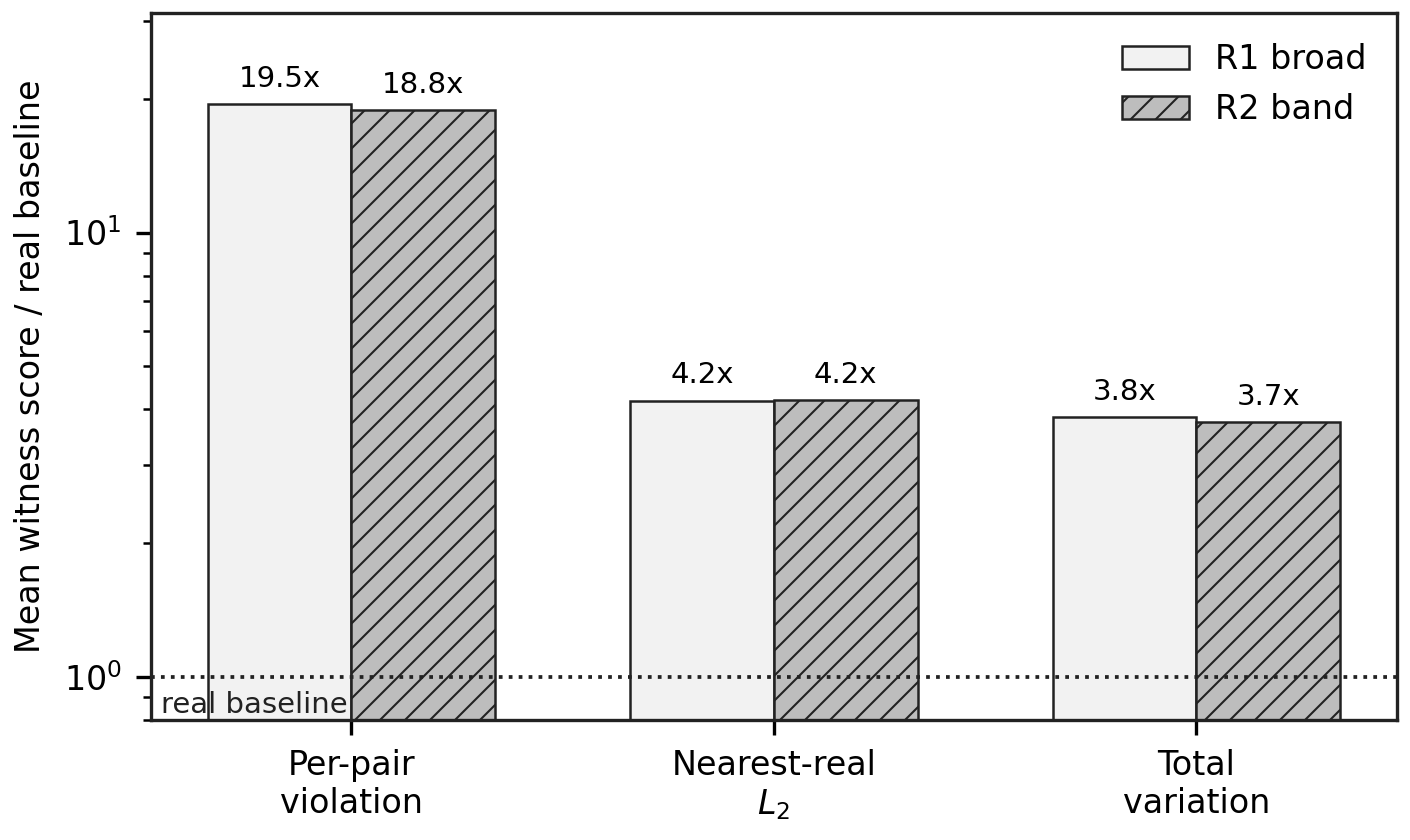
\includegraphics[width=\columnwidth]{lard_witness_audit_ratios.png}
\caption{LARD witness-audit ratios for the broad SAT witnesses. Values are means over recovered witnesses divided by the held-out real-image baseline. The $R_1$ and same-extent $R_2$ witnesses are valid pixel vectors, but they are about $19\times$ above the real per-pair violation baseline, $4\times$ farther from nearest same-class held-out images, and nearly $4\times$ higher in total variation.}
\label{fig:lard_audit_ratios}
\end{figure}

\subsection{Convolutional front-end scalability probe}
\label{sec:conv_probe}

As an architecture-boundary check, we trained a small ReLU CNN on the TinyTaxiNet regression task (\texttt{Conv$\to$Conv$\to$FC}, test CTE MAE $1.40$\,m), exported it to ONNX, and ran the P3 CTE-bound subqueries through the same region-tagged workflow on eight centered anchors. The broad pixel-ball queries produce $12$ SAT and $2$ UNSAT verdicts; two additional subqueries return non-SAT/UNSAT Marabou status codes recorded as solver errors by the exact parser. The local-PCA queries produce $14$ UNSAT, $1$ SAT, and $1$ timeout at the 300\,s budget. The probe shows that the workflow can be applied to a convolutional front end, but the result is a measured scalability boundary rather than a new transfer claim: no matched random control was run for this CNN, and the conv-AE P1a/P1b queries time out at the reported budget.

\subsection{Prior-Result Cross-Checks}
\label{sec:prior_cross_checks}

These directional consistency checks compare the region-tagged verdicts with prior results and the released dataset. Where regimes overlap, the region-tagged verdicts are directionally consistent with prior TaxiNet-family results: P3 at $\varepsilon{=}0.02$ ($892/893$ verified) is directionally consistent with Julian et al.'s adaptive stress testing, which finds no failure at $\delta_\text{max}{=}0.02$ (its failure threshold is $|d|{>}10$\,m from the centerline)~\cite{julian2020}; the P4 wrong-sign rate of $1.7\%$ ($142/8{,}227$, $95\%$ Wilson CI $1.47$--$2.03\%$) recomputes independently on the released dataset and contrasts with Pasareanu et al.'s zero blatant left/right confusion on the experimental Boeing TaxiNet~\cite{pasareanu2023closedloop}, so the wrong-sign mode is TinyTaxiNet-specific; P1d's box-abstraction-artifact status is empirically attested by the dataset (empirical max $|\mathrm{HE}_\text{err}|=62.6^\circ$, well below the $90^\circ$ threshold). The empirical-baseline reproducer script is released with the artifact.

% ============================================================
\section{Witness Audits and Region Stress Tests}

For the main regional SAT results P1 and P4, we analyze representative unconstrained and mean-constrained witnesses for plausibility. P2 and P3 produce many SAT witnesses (one per nominally fragile image at each $\varepsilon$); their structure is captured by the verification rates and per-image categorization in Section~\ref{sec:p3_results} and the P2 summary in Section~\ref{sec:p2_supporting}.
The witness audit does not modify Marabou's SAT/UNSAT verdict; it reports empirical support signals for recovered SAT witnesses. We use the audit as a triage rule rather than a realism certificate. A witness that appears only in a broad pixel region and scores poorly on all support signals is treated as an abstraction-driven candidate. A witness that survives data-conditioned regions and is also observed directly in data, or re-rendered in a domain with a known renderer, is treated as dataset- or semantic-supported. Mixed audit signals remain unresolved and indicate where additional data, a stronger image generator, or a physical rendering model is needed.

\subsection{Pixel-box witnesses}
\label{sec:box_coverage}
\label{sec:plausibility_constrained}

The two unconstrained witnesses (P1a, P4 left) violate $\text{mean}(x) = 0.5$ (witness means $0.611$ and $0.472$) and are inconsistent with the released preprocessing invariant. Both failure modes survive the mean constraint with witnesses that satisfy the invariant: P1a at $\text{CTE}{=}10.0$, and P4-left as a wrong-sign SAT with achievable magnitude $\text{CTE}\le-20$ in the released threshold sweep. Across the P1a and P4 mean-constrained counterexamples, the nearest real images are at $L_2$ distances of $1.6$--$1.8$, indicating that counterexamples combine pixels from different images in ways that do not occur in the dataset but are permitted by the per-pixel box abstraction.

The pixel-box is tight per-pixel but admits vastly more pixel \emph{combinations} than the training distribution exhibits: $0\%$ of real images have more than half their pixels within $20\%$ of the box width of either per-pixel bound, and the formal P6 bound is $4.86\times$ wider in CTE than the empirical centered range. Mean-constrained SAT survival (Section~\ref{sec:p1_results}, P1a/P1b/P4 all remain SAT under $\text{mean}(x){=}0.5$) shows the failures are not artifacts of the missing mean invariant; the P4 wrong-sign mode is empirically present on $1.7\%$ of offset images independent of any adversarial construction. A first attempt to tighten the region with linear statistical constraints (global PCA box on all 128 principal directions, $95\%$ TV bound, $95\%$ per-row mean bands) left P1a, P1b, P4 all SAT, which motivates the nonlinear autoencoder-composed region introduced next.

\textbf{Autoencoder-composed verification.} The first nonlinear tightening step is the AE decoder-box abstraction. Its construction (subset-specific autoencoder, decoder composed with TinyTaxiNet, latent bounding box, mean-sum auxiliary output) is described in Section~\ref{app:construction_ref}. For each property we apply the relevant subset autoencoder ($\mathrm{AE}_\text{centered}$ for P1, $\mathrm{AE}_\text{left}$ and $\mathrm{AE}_\text{right}$ for P4) and verify the negated postcondition over the composed network with $\text{mean}(x) = 0.5$ enforced. Table~\ref{tab:plausibility_constrained} reports the pixel-box and AE-composed verdicts side by side.

\begin{table*}[htbp]
\centering
\sttttablefont
\setlength{\tabcolsep}{6pt}
\begin{tabular}{lll}
\toprule
Query & Pix+mean & AE+mean \\
\midrule
P1a (CTE$\ge$10) & SAT & \textbf{UNSAT} \\
P1b (CTE$\le${-}10) & SAT & \textbf{UNSAT} \\
P4 left, base (CTE$\le$0) & SAT (boundary witness; magnitude floor $\le -20$) & SAT, $0.00$ \\
P4 left, sweep (CTE$\le$$-$3) & --- & SAT, $-$3.42 \\
P4 right, base (CTE$\ge$0) & SAT, 0.00 & SAT, 0.00 \\
P4 right, sweep (CTE$\ge$$+$3) & --- & SAT, $+$3.00 \\
\bottomrule
\end{tabular}
\caption{Pixel-box versus AE-composed verification, both with $\mathrm{mean}(x)=0.5$ enforced. Base rows use the original property negation; sweep rows tighten the wrong-sign magnitude threshold.}
\label{tab:plausibility_constrained}
\end{table*}

\textbf{Autoencoder support audit.} The AE-composed region has a measured abstraction-distortion budget. Train-only latent boxes cover $\ge 97.8\%$ of held-out latents across the centered, left, right, and off-center subsets. Median reconstruction $L_\infty$ is $0.118$--$0.160$; median prediction shift is $0.66$--$0.77$\,m for CTE and $2.20^\circ$--$3.79^\circ$ for HE, with p95 shifts of $2.35$--$2.91$\,m and $7.59^\circ$--$11.69^\circ$. The companion classifier accepts $86.7$--$97.3\%$ of random latent-box decodes as ``real,'' making it a permissive support screen. Pixel-box witnesses fall outside both screens (classifier logits $-8$ to $-32$); AE-composed witnesses score inside the classifier-supported region (logits $+2.63$ to $+5.03$).

The AE decoder has linear output pixels, so we audit the decoded range of stored witnesses. The mean-constrained P4 AE witnesses remain inside the valid pixel cube: the strongest stored left witness has decoded range $[0.236,0.842]$, and the stored right witnesses at $+2$\,m and $+3$\,m have ranges $[0.198,0.767]$ and $[0.243,0.761]$. Random latent-box controls also stay fully in $[0,1]^{128}$ for 100.0\%, 99.1\%, 98.6\%, and 98.3\% of centered, left, right, and off-center decodes, respectively. P1a/P1b have no AE witness to audit because those decoder-box queries are UNSAT.

\textbf{Autoencoder stability analysis.} Latent-box quantile sweeps, nearest-neighbor checks for $\pm3$\,m P4 witnesses, and retraining at seeds 7 and 13 leave the AE-composed verdict pattern unchanged. The released artifact includes the scripts and outputs for these stability checks.

\subsection{Learned-support results}

The AE-composed reruns produce three results:

\begin{itemize}[nosep]
  \item \textbf{P1 (output bound).} Under the subset-specific $\mathrm{AE}_{\text{centered}}$ learned decoder-box abstraction with $\text{mean}(x) = 0.5$ enforced, P1a and P1b are UNSAT (Table~\ref{tab:plausibility_constrained}), and the CTE$= \pm 10$ pixel-box witnesses do not correspond to inputs in this abstraction. The support audit above quantifies the decoder budget, including reconstruction-induced prediction shift and reconstruction $L_\infty$ reaching $0.27$.
  \item \textbf{P4 (directional correctness).} Wrong-sign behavior appears both in the dataset and in the AE-composed verification runs: 1.7\% of \emph{offset} images ($|\text{CTE}|{>}2$\,m, 142/8{,}227) produce wrong-sign CTE, and the AE-composed queries return SAT witnesses at $\pm 3$\,m within the subset-specific learned decoder-box abstractions. The AE witnesses are not direct copies of empirical wrong-sign images (L$_2$ distance $\geq 0.86$ from nearest real images), but the observed and verified magnitudes are consistent.
  \item \textbf{Conv-AE rerun.} Retraining the AE family with Marabou-compatible convolutional decoders reproduces the FC P4 SAT verdict. P1a/P1b time out at the $600$\,s budget, so the FC AE's P1a/P1b UNSAT is specific to the tested FC decoder-box region within this verification budget.
\end{itemize}

The per-seed autoencoder weights are released for reproducibility.

\subsection{Math-encoded regions}
\label{sec:math_regions}

\textbf{Math-encoded regions.} The math-encoded region family $R_6$ intersects $R_2$ with linear-in-pixel constraints calibrated from empirical quantiles of the released dataset: total variation, Fourier high-frequency $L_1$, photometric basis residual, per-row mean, per-cell mean, and per-pair Lipschitz bounds. Across the tested calibrations:

\begin{enumerate}[nosep]
  \item \emph{No tested math region eliminates the failure mode.} P1a/P1b, P4-left, and P4-right remain SAT under the main math-region calibrations: box$+$mean, TV~$\le 10$, Fourier HF-$L_1\le 3.34$, and photometric residual~$\le 0.184$. An explicit threshold sweep on P4-left shows wrong-sign witnesses exist at $\text{CTE}\le -20$\,m under every tested region, including TV~$\le 2$ and Fourier~$\le 0.62$ (both well below the empirical centered minimum).
  \item \emph{The only SAT$\to$UNSAT flip is over a region containing no real centered samples.} Tightening Fourier to $\tau\le 0.62$ (orthonormal, $\sim 10\times$ below the centered minimum HF-$L_1$) flips P1a/P1b to UNSAT, but the region admits $0/893$ real centered images, so the UNSAT proves the queried output bound only over that empty-on-data slice of the input space. The released artifact records the Fourier unit reconciliation.
  \item \emph{The witness audit rejects most math-region witnesses.} On the 91 math-region SAT witnesses for which the full pixel vector is stored, the original classifier scores $86/91$ below probability $0.1$ ($94.5\%$; $95\%$ Wilson CI $87.8$--$97.6\%$), and a disjoint-split retrained classifier scores $69/91$ below $0.1$. The median nearest-real-image $L_2$ distance is $1.41$ (typical real-to-real $\sim 0.8$ on the centered subset), and the per-pair Lipschitz violation fraction is an order of magnitude above the centered-baseline rate of $0.009$ on box-only witnesses and remains elevated on generic-math witnesses.
\end{enumerate}

\textbf{Classifier-calibration audit.} The classifier is used as a support screen, and its calibration is checked three ways. The original classifier accepts $97.5\%$--$98.6\%$ of released real images across the centered, left, right, and off-center subsets, but these are training-set acceptance rates. A disjoint-split retraining accepts $98.9\%$ of 1{,}000 never-seen real images and still rejects most math-region witnesses: median probability $2\times 10^{-4}$, $69/91$ below $0.1$, $11/91$ above $0.5$. A fifth fake-family stress test with smooth low-frequency synthetic images shows the classifier's limits: the original classifier rejects $70.9\%$ below $0.1$ and admits $19.2\%$ above $0.5$, while the disjoint-split classifier rejects $43.9\%$ below $0.1$ and admits $36.4\%$ above $0.5$.

The three audit signals measure different support axes. Math-region witnesses have low classifier scores together with elevated nearest-image distance and per-pair violations; TinyTaxiNet $R_5$ label-box witnesses are much closer in nearest-image distance but are often rejected by the classifier; MNIST nearest-image distance is close to its real-digit baseline, while classifier and per-pair signals remain discriminating. The audit reports disagreement among support proxies alongside agreement.

Exact constraint definitions and Marabou slack-variable encodings are in Appendix~\ref{app:construction_ref}; script names, runway-layout variants, combined-constraint runs, and sensitivity reruns are released with the artifact.

\textbf{Additional reruns.} The released artifact includes math-region sweeps, runway-calibrated variants, P1-patterned and AE intersections, calibration-quantile checks, stratified witness audits, and failure-hardness curves.

Under the original plausibility classifier, the real-centered baseline has median probability 0.991 and mean probability 0.934, with 41/45 images above 0.5. The 91 math-region SAT witnesses have median probability 0.000 and mean probability 0.035, with only 3/91 above 0.5; the disjoint-split retraining sensitivity is reported above.

% ============================================================
\section{Comparison with Prior Work}
\label{sec:prior_work}

\subsection{Region tightness and empirical support}

Comparable verification approaches differ primarily in how they define the verifier's input set and how much support that set has in the image source being modeled. Mitra et al.~\cite{mitra2024visionsurvey} taxonomize vision-based autonomous-system verification along a related axis: perception NN alone, camera-plus-NN composition, or full closed loop. The Marabou pixel-box approach, used for the baseline P1, P3, P4, and P6 queries here and by Wu et al.\ for per-image $L_\infty$ balls, is sound and complete over its encoded region but admits non-physical pixel combinations. VerifyGAN~\cite{katz2022} sits at the opposite end: every verifier input lies in the learned generator range, but the guarantee is incomplete relative to real images outside that range. Activation-pattern partitioning~\cite{kadron2021}, local-PCA regions, and the subset-specific autoencoder used here sit between those endpoints. Simulation-based falsification is a complementary, non-formal counterpart: Fremont et al.~\cite{fremont2020} use VerifAI to analyze and redesign a TaxiNet-family taxiing network by searching for failures in closed-loop simulation rather than proving properties over an encoded region. Elboher et al.~\cite{elboher2024runway} provide the closest recent runway-domain Marabou comparator outside TinyTaxiNet: they verify an Airbus runway-object classifier under noise, brightness, contrast, and combined image perturbations, and reduce the number of robustness queries by exploiting monotonicity across perturbation strengths. Table~\ref{tab:prior_work} positions this work against the most directly related runway and TaxiNet-family verification studies.

\begin{table*}[t]
\centering
\sttttablefont
\setlength{\tabcolsep}{4pt}
\begin{tabular}{>{\raggedright\arraybackslash}p{1.9cm}>{\raggedright\arraybackslash}p{2.3cm}>{\raggedright\arraybackslash}p{2.0cm}>{\raggedright\arraybackslash}p{2.6cm}>{\raggedright\arraybackslash}p{2.3cm}>{\raggedright\arraybackslash}p{2.3cm}}
\toprule
Work & Input region & Network verified & Plausibility strategy & Main guarantee & Main limitation \\
\midrule
Kadron et al.\ (VSTTE'21) & Prophecy-patterned per-sequence pixel boxes & TinyTaxiNet & Activation-pattern preconditions reduce loose pixel corners & 33/111 time-interval sequences proved under $|y_0|<10$\,m & Some partitions too broad to prove; soundness still relative to pixel box \\
Katz et al.\ (VerifyGAN, JAIS'22) & 2-D state cell $\times$ 2-D GAN latent box & GAN generator $\circ$ TinyTaxiNet & Generator range defines the verifier inputs & Correctness band over state/latent cells & Real images outside generator support are outside the guarantee; verifies a composed network \\
Wu et al.\ (FMCAD'20) & $L_\infty$ ball around individual pre-processed images & TinyTaxiNet & None; per-image local robustness & Per-image robustness with Marabou parallelization & No regional plausibility or global behavior claim \\
Elboher et al.\ (DASC'24) & Per-image perturbation regions: noise, brightness, contrast, and combinations & Airbus runway-object classifier & Perturbation family defined by image operation & Robustness assessment with nearly 60\% fewer queries using monotonicity & No learned-support region or witness-support audit \\
This work & Six tagged regions: pixel boxes, mean invariant, AE decoder box, local PCA, label-conditioned box, linear diagnostic filters & TinyTaxiNet; subset decoder $\circ$ TinyTaxiNet for $R_3$ & Region tags plus witness audit with classifier, nearest-neighbor, and Lipschitz signals & Verdict flips across regions; dimension/direction decomposition; P4 persists with empirical support & All guarantees are region-relative; AE and classifier are fitted support models \\
\bottomrule
\end{tabular}
\caption{Comparison with directly related runway and TaxiNet-family verification studies.}
\label{tab:prior_work}
\end{table*}

\subsection{Direct Runway and TaxiNet-Family Comparisons}

\textbf{Elboher et al.\ (DASC 2024).} Verify an Airbus runway-object classifier with Marabou under three image-perturbation families: pixel noise, brightness, contrast, and selected combinations. Their study is the closest runway-domain Marabou comparator: it verifies a larger industrial classifier and shows that robustness depends strongly on the perturbation family, with noise producing weaker robustness than brightness or contrast. Their main engineering contribution is query reduction: monotonicity across perturbation strengths and reuse of previous results reduce the number of verifier invocations by nearly 60\%. The present work addresses a complementary layer of the same workflow: each verdict is tagged with the encoded region, learned/local/box/linear-filter regions are compared on a fixed property set, and recovered witnesses are audited for dataset support. Thus Elboher et al.\ show that perturbation-region choice matters on an industrial runway classifier; this paper provides the region-tagging and witness-audit machinery for deciding how much support a SAT witness has under the chosen region.

\textbf{Kadron et al.\ (VSTTE 2021).} Verified TinyTaxiNet against $|y_0| < 10$\,m (which we adopt as one P1 sub-query) using Marabou under preconditions combining Prophecy-mined activation patterns with per-sequence pixel boxes; correctness thresholds ($1.0$\,m CTE, $5^\circ$ HE, which we adopt for P2) were evaluated on Boeing TaxiNet rather than TinyTaxiNet because Marabou could not handle the Boeing architecture's combination of convolutions and eLU activations. They report Marabou proofs for 33 of 111 time-interval sequences with $\ge 5$ images (longest proved sequence: 17 images); our P1-patterned replication is single-image rather than per-sequence and verifies 16 of 24 observed centered patterns. Both reflect the same mechanism: tighter per-partition boxes eliminate non-physical corners that a global pixel box admits. Section~\ref{sec:plausibility_constrained} extends the same intuition nonlinearly via autoencoder composition.

\textbf{Katz et al.\ (VerifyGAN, JAIS 2022).} Move verification out of pixel space by composing a conditional GAN with TinyTaxiNet and verifying over a 4-D box that pairs a 2-D state cell (CTE, HE) with the 2-D latent $L_\infty$ ball, with the state space partitioned into $16{,}384$ cells and the latent truncated to $[-0.8, 0.8]^2$. Every input Marabou considers is GAN-generated by construction, so non-physical pixel combinations are excluded. Soundness is relative to the GAN-generated image set, not the underlying real-image distribution. Their pipeline verifies a different network (GAN$\circ$TinyTaxiNet) over a different input space (the 4-D state-plus-latent box vs.\ our $128$-D pixel-box and AE-composed regions), so direct numerical comparison is not possible. Our AE-composed region (Section~\ref{sec:plausibility_constrained}) is a ReLU-only learned-support analogue: cheaper to integrate into Marabou than a full GAN, at the cost of a looser decoder-box (reconstruction $L_\infty$ up to $0.27$).

\textbf{Wu et al.\ (FMCAD 2020).} Studied local robustness queries on TinyTaxiNet using Marabou v1.x with a focus on parallelization (Split-and-Conquer); the input region is a per-image $L_\infty$ ball and the postcondition is local robustness, with no plausibility step. Our P3 setup is the closest analogue and is complementary: we use Marabou~2.0 (queries solve without explicit Split-and-Conquer scheduling on this small network), evaluate at three dataset-calibrated $\varepsilon$ values rather than one, and report both 20-image diagnostics and full centered-subset rates ($n{=}893$). Qualitatively consistent: more violations at tighter bounds.

\subsection{Broader Verification Landscape}

This work sits in the deterministic, region-aware, perception-layer quadrant. Pixel-space verifiers~\cite{liu2019algorithms,singh2019deeppoly,wang2021betacrown,bak2020nnenum} take region selection as user-supplied; closed-loop NN-controlled-system verifiers~\cite{tran2020nnv,ivanov2021verisig,julian2021reachability,ainncs2020} sidestep pixel boxes by working in state space but assume the NN takes a state input; the ML-security thread (randomized smoothing~\cite{cohen2019smoothing}, semantic-perturbation layers~\cite{mohapatra2020semantify}, spatial-robustness studies~\cite{engstrom2019spatial}) arrives at the same region-choice problem from the training side. Against the most directly comparable runway and TaxiNet-family approaches (Table~\ref{tab:prior_work}): Wu et al.\ change \emph{how} queries are solved at scale; Elboher et al.\ reduce repeated image-perturbation queries on an industrial classifier; Kadron et al.\ shrink the pixel box via activation-pattern partitioning; Katz et al.\ replace it with a GAN-defined latent abstraction. This work tags, compares, and audits verdicts across multiple abstractions on the same property set.

\textbf{State-to-image verification.} The most directly comparable predecessor is Yang and Rinard's Tiler~\cite{yang2022tiler}, which verifies a camera-centerline regression network on a synthetic ray-traced road scene by formalizing the feasible input space as the image of an explicit observation process $g{:}\, \mathcal{S}{\to}\mathcal{P}(\mathcal{X})$ from a low-dimensional state space (camera offset $\delta$, viewing angle $\theta$) to $32{\times}32$ grayscale images, then tiling $(\delta,\theta)$ and verifying per-tile robustness via MILP. The setting is close to ours: camera-derived perception of a road centerline and regression of an offset and angle. The main differences are dataset source (idealized ray-tracing vs.\ X-Plane simulator), network class (ConvNet vs.\ ReLU MLP), and verifier (MILP-per-tile vs.\ Marabou with multiple explicit region constructions). Tiler defines one observation-process-induced region and decomposes it over a $(\delta,\theta)$ grid; our protocol treats the region itself as the experimental variable and runs the same property set under six alternatives ($R_1$--$R_6$). Tiler's state-conditioned image set is the kind of region our $R_3$ (autoencoder decoder-box) and $R_4$ (local-PCA) regions approximate when no ray-traced observation model is available.

\textbf{Geometric-perturbation verification.} Estornell et al.~\cite{estornell2025visual} address the same input-support gap from the verification side: they construct a boundable state-to-image mapping using per-entity geometric transformations (translation, rotation, scaling, plus brightness/contrast modeled as an affine pixel-intensity map), propagate pixel-wise bounds through the controller using DeepG and CROWN-style linear-relaxation perturbation analysis (LiRPA), and produce closed-loop outer-approximations of reachable sets on CartPole, Pendulum, and Acrobot Gym environments with explicit soundness guarantees. Their pipeline gives stronger guarantees than data-conditioned regions but requires entity-decomposable scenes and an analytic state-to-observation model at verification time. We work in the regime where only a dataset and statistical region models are available. In that setting, each verdict must be tagged with the region construction that produced it, and each recovered witness must be interpreted together with its audit signals.

\textbf{Verification and validation of abstractions.} Peper, Miao, Mitra, and Ruchkin~\cite{peper2025unifiedVV} recently propose a unified verification-and-validation pipeline for vision-based autonomy in which an Interval-MDP abstraction is first model-checked at confidence $1{-}\beta$ and then statistically re-validated on a held-out dataset $D_{\mathrm{val}}$ under environment shift, yielding nested probabilistic guarantees on the abstraction's continued validity. Their validation target is the IMDP abstraction, a model used as input to verification; our audit target is the individual solver-returned witness. Both approaches treat empirical checking of verification artifacts as part of the verification workflow, but they operate at different levels: abstraction-level statistical validation in their case, witness-level audit in ours. Mitra et al.~\cite{mitra2024visionsurvey} taxonomize the vision-based verification subfield in a Festschrift survey chapter; the present work instantiates one row of that taxonomy, DNN perception with SMT-based verification, with a multi-region comparative protocol and witness audits.

\textbf{Position of this work.} The input-support gap for pixel-space verification is well recognized, and constructive sound regions exist where a parametric observation, generator, or latent model is available (Tiler, Estornell et al., VerifyGAN, NNLander-VeriF~\cite{santacruz2022nnlander}, SEVIN~\cite{parameshwaran2025sevin}). SEVIN learns a VAE latent space and verifies image-controller properties over annotated convex polytopes; it is a constructive single-region method, while this work compares multiple region constructions on a fixed property set. Geng et al.~\cite{geng2023nap} make a related argument that ``data as specification is too tight'' as motivation for Neural Activation Patterns, a delta-relaxed per-class subset-pattern construction distinct from our P1-patterned region, which uses full per-image Prophecy-style patterns~\cite{kadron2021,prophecy2019}. Auditing solver-produced counterexamples is also a recognized concern: Song et al.~\cite{song2018unrestricted} construct \emph{unrestricted adversarial examples} entirely from a generative model's latent space, and Barredo-Arrieta and Del Ser~\cite{barredoarrieta2020plausible} audit classifiers by generating \emph{plausible counterfactuals} through a GAN under a multi-objective trade-off between model confusion and human plausibility.

Building on this literature, this work contributes the operational layer for region-relative interpretation: a reusable Marabou protocol that tags each verdict with one of six explicit region constructions, reruns a fixed property set across those constructions, and audits recovered witnesses with one learned and two non-learned dataset-support signals. The main TinyTaxiNet case study supplies the detailed property analysis; the MNIST, external \texttt{mnist\_fc}, LARD, and controlled-oracle runs exercise the same protocol outside the original simulator setting. The empirical findings follow from that protocol: matched random-subspace controls show that high verification rates in learned low-dimensional regions can be driven by dimensionality; data-aligned local-PCA regions recover witnesses that random 8D regions miss; most math-feasible witnesses fail both classifier audits; and the apparent CTE/HE asymmetry is isolated to postcondition headroom by a closed-form first-order Jacobian diagnostic and a controlled postcondition-bound sweep that erases the asymmetry once headroom is equalized across axes.

% ============================================================
\section{Reproducibility and Runtime}
\label{sec:reproducibility}

\subsection{Reusable module and instantiations}
\label{sec:module}

The transferable artifact is \texttt{region\_audit.py}, a reusable implementation of the six region constructors and three witness-audit signals for flattened image-input networks verified through the \texttt{maraboupy} API. The module is parameterized by image grid shape and calibration data. Its interface has four parts:

\begin{itemize}[nosep]
  \item \textbf{Region constructors.} \texttt{r1\_subset\_box} ($R_1(S)$), \texttt{r1\_linf\_ball} ($R_1(x_0,\varepsilon)$), two $R_3$ decoder constructors for in-query ReLU decoders or pre-composed decoder networks, \texttt{r4\_local\_pca} ($R_4$), and \texttt{r5\_neighbor\_box} ($R_5$). Each returns a tagged \texttt{Region} whose \texttt{attach(net, ivars)} adds its bounds and constraints to a Marabou network.
  \item \textbf{Intersectable constraints.} \texttt{mass\_equality} and \texttt{mass\_band} (the $R_2$ layer, exact invariant or statistical band), and the $R_6$ family: \texttt{tv\_bound}, \texttt{fourier\_hf\_bound}, \texttt{photometric\_bound}, \texttt{per\_pair\_bound}, \texttt{per\_row\_mean\_band}, all linear-in-pixel using the slack-variable encoding of Appendix~\ref{app:construction_ref}. \texttt{intersect(region, \ldots)} composes any of them with any region under a new tag.
  \item \textbf{Tagged queries.} \texttt{run\_query(make\_net, region, postcondition)} builds a fresh network, attaches the region, applies the negated property (helpers: \texttt{output\_at\_least}, \texttt{output\_at\_most}, \texttt{class\_confusion}), solves, and returns the verdict together with the region tag, its calibration parameters, and the witness vector when SAT. Region tagging is part of query execution and result serialization.
  \item \textbf{Witness audit.} \texttt{WitnessAudit} calibrates the per-pair Lipschitz thresholds from reference images and scores any witness vector with the three signals; \texttt{baseline()} reports the same signals on real images, so witness scores are always read against a same-domain reference. \texttt{load\_relu\_classifier} adapts the small ReLU plausibility classifiers used in both case studies; any callable returning a probability can be substituted.
\end{itemize}

An instantiation supplies dataset loading, subset predicates, neighbor rules, calibration data, and the network reader. The two released adapters, \texttt{taxinet\_instantiation.py} and \texttt{mnist\_instantiation.py}, also serve as smoke tests: 8/8 TinyTaxiNet checks and 7/7 MNIST checks reproduce representative recorded verdicts through the module, including the in-Marabou class-AE decoder composition. The per-experiment scripts remain the source artifacts for the paper's numerical results; the module packages the same constructions for reuse.

\subsection{Artifact contents}

The code, verification-result JSONs, reusable module, smoke tests, and baseline VNN-LIB query export are publicly available at \url{https://github.com/Jireh1226/tinytaxinet-marabou-verification}; the final submission artifact records the exact commit hash. Large model artifacts (\texttt{.npz}, \texttt{.keras}, \texttt{.onnx}, \texttt{.h5}) are regenerated by released scripts. The TinyTaxiNet weights and \texttt{SK\_DownsampledGANFocusAreaData.h5} dataset are obtained from the upstream Stanford Intelligent Systems Laboratory \texttt{sisl/VerifyGAN} repository and are not redistributed. The environment is Python~3.11.14 with \texttt{maraboupy}~2.0.0, \texttt{numpy}, \texttt{h5py}, \texttt{tensorflow}, \texttt{tf2onnx}, and \texttt{matplotlib}; experiments were run on laptop-class macOS CPUs, with no GPU used for the LARD run. Marabou uses per-query timeouts only, with \texttt{normalize=False} for the \texttt{.nnet} reader.

A tiered \texttt{Makefile} separates empirical, solver, and learned-model reproduction. \texttt{make reproduce-empirical} recomputes TinyTaxiNet empirical summaries, Jacobian/headroom diagnostics, the controlled postcondition sweep, and classifier-support audits using only \texttt{numpy} and \texttt{h5py}. \texttt{make reproduce-solver} adds \texttt{maraboupy} for representative verdicts and exact-solver checks. \texttt{make reproduce-learned} runs the MNIST/TensorFlow components. \texttt{make reproduce-headlines} runs the first two tiers, so every TinyTaxiNet headline number is reproducible without TensorFlow.

The baseline query set is exported as 118 \texttt{.vnnlib} files in standard SMTLIB2 format with an \texttt{instances.csv} model map. Mean-constrained, local-PCA, AE-composed, math-region, classifier, threshold-sweep, controlled-oracle, MNIST, external \texttt{mnist\_fc}, and LARD follow-ups are released as Python scripts plus matching JSON outputs; the artifact manifest maps each experiment to its script and output files.

\subsection{Runtime}

All 474 baseline queries complete within the 1-hour timeout: P1-patterned (96), P2 (160), and P3 (160) resolve at $\sim$10--20\,ms per query (totals under 3\,s); P4 is sub-second; P6's 52 binary-search queries take 70\,s total. Peak memory is 80--108\,MB. The expanded local-PCA P3 run over all 893 centered images takes 1742\,s at $1\sigma$ and 2760\,s at $2\sigma$ with a 300\,s per-sub-query timeout; the deterministic 200-anchor $3\sigma$ run takes 1096\,s. The full-centered-subset reruns of P2 and P3 mean$+$clip complete in 183\,s total wall-clock time across all $\sim 8{,}000$ sub-queries. The follow-up math-region, sensitivity-rerun, stratified-audit, and threshold-sweep experiments complete in tens of seconds to a few minutes each; the most expensive single experiment is the conv-AE P1a/P1b query, which times out at the chosen $600$\,s budget on both centered sub-queries.

% ============================================================
\section{Calibration Checks}
\label{sec:calibration}

Two small calibration checks exercise the implementation rather than serving as additional case studies in Table~\ref{tab:evidence_map}. First, a deterministic 20-instance slice of the VNN-COMP \texttt{mnist\_fc} benchmark is solved with the same Marabou~2.0 binary and VNN-LIB handling used in the paper; $12$ instances complete within the budget and all $12$ match the published SAT/UNSAT label, with zero disagreements. Second, a renderer-controlled lane-image domain with known ground truth verifies three constructed ReLU models: a correct model, an injected true-failure model, and an artifact-trigger model. Broad boxes are SAT for all three, while the manifold-constrained local-PCA region removes the artifact failures and preserves the injected true failure; the nearest re-rendered state reproduces wrong-sign only for the injected true-failure model. This calibration also shows why the audit is not used as a single-threshold oracle: per-witness distance and classifier-like support signals alone do not separate all true and artifact cases, while the combination of region survival and re-rendered empirical support does. These checks calibrate solver/property plumbing and the witness-audit interpretation; the main evidence for the paper remains the TinyTaxiNet case study plus the MNIST, \texttt{mnist\_fc}, and LARD instantiations above.

% ============================================================
\section{Discussion and Validity Scope}
\label{sec:limitations}

We separate the scope of the results into two categories: conditions affecting the \emph{soundness of the encoded verification problem} (whether the SAT/UNSAT verdicts are correct on the input region as encoded), and conditions affecting \emph{external validity} (whether the input region as encoded reflects the deployed system).

\subsection{Soundness of the Encoded Verification Problem}

\begin{enumerate}[nosep]
  \item \textbf{Binary-search tolerance.} P6 binary-search bounds are accurate to $\pm 0.01$, not the exact extrema. The reported envelope is therefore an axis-aligned outer envelope to within this tolerance.
  \item \textbf{Latent decoder-box restriction.} The AE-composed UNSAT in Section~\ref{sec:plausibility_constrained} is sound with respect to the learned decoder applied to the latent bounding box of training encodings, with $\text{mean}(x) = 0.5$ enforced. Images outside the decoder range are outside the guarantee, and the decoder's reconstruction $L_\infty$ reaches 0.27 in the worst case. The P1a/P1b decoder-box flip is an 8D in-region result. The matched random-8D affine control in Section~\ref{sec:p1_results} reproduces the flip, so this particular result is attributed to low dimensionality rather than decoder-specific support.
  \item \textbf{Plausibility classifier scope and permissiveness.} The classifier is trained to discriminate real images from four synthetic fake types: per-pixel-box corners, cross-image blends, uniform noise, and high-frequency patterns. The original classifier's real-image acceptance is a training-set rate; the disjoint-split retrained classifier and the fifth fake-family stress test in Section~\ref{sec:math_regions} report the held-out and out-of-family behavior. The classifier also accepts most random AE latent-box decodes as ``real'' (Section~\ref{sec:plausibility_constrained}). We therefore use classifier score as one dataset-support proxy, alongside nearest-neighbor distance and per-pair Lipschitz violation fraction.
  \item \textbf{Prediction shift under AE reconstruction.} The AE support audit in Section~\ref{sec:plausibility_constrained} quantifies the CTE/HE prediction shifts induced by reconstruction. AE-composed verdicts therefore characterize the network's behavior on the AE-reconstructed image set, not pixel-identical inputs; UNSAT under the AE region does not, by itself, rule out failure on the actual centered image.
  \item \textbf{Multi-seed scope.} Multi-seed stability was tested over three autoencoder training seeds (42, 7, 13). Architecture choice, latent dimension, train/validation split, classifier seed, and classifier architecture are fixed. The reported stability covers SAT/UNSAT agreement and within-0.42\,m witness magnitudes across these three seeds.
  \item \textbf{Local-PCA support-model scope.} The local-PCA region uses $d=8$, radius $\alpha$, and same-state-neighbor bins as modeling parameters. The top-8 directions capture about $92\%$ of same-state-neighbor deviation variance, leaving 5--11\% outside the verified subspace depending on the anchor. These verdicts therefore characterize the encoded local linear region, not the full same-state image set.
  \item \textbf{Matched-dimension control scope.} The TinyTaxiNet P3 random-subspace control decomposes verification-rate gain into dimension and direction effects, and matched random 8D controls are now also run for VNN-COMP \texttt{mnist\_fc} ($450/450$ UNSAT at $1/2/3\sigma$) and LARD ($900/900$ UNSAT across bounded and unbounded variants). In all three settings, a random subspace at matched scale removes broad witnesses at least as completely as local PCA. The P1a/P1b AE decoder-box flip is likewise reproduced by a random 8D affine region at $d{=}8$, and a P3 dimension sweep ($d\in\{2,\dots,64\}$) locates the PCA/random divergence at $d\gtrsim16$. All controls use three seeds; extending the decomposition to more networks, properties, and subspace dimensions, and to deeper high-$d$ solver budgets, remains future work.
  \item \textbf{Math-region filter scope.} The TV, Fourier, photometric, and per-pair-Lipschitz constraints of Section~\ref{sec:math_regions} are linear-in-pixels filters calibrated on the centered runway subset. Math-feasible witnesses are audited downstream, and Section~\ref{sec:math_regions} reports the original and disjoint-split classifier counts. The released P4-left threshold sweep also shows wrong-sign witnesses at $\text{CTE}\le-20$\,m under every tested math region, including settings below the empirical centered-subset minimum on each calibration quantity.
\end{enumerate}

\subsection{External Validity to Deployed Systems}

\begin{enumerate}[nosep]
  \item \textbf{Hyperrectangular over-approximation.} Per-pixel boxes in $R_1$--$R_2$ admit non-physical pixel combinations. SAT counterexamples in $R_1$ need not be supported by the runway-image distribution; this is the core motivation for the AE-composed region $R_3$. Activation-pattern partitioning (P1-patterned) mitigates this for centered images but does not remove the region-relative scope.
  \item \textbf{Preprocessing-invariant modeling.} Follow-up mean-constrained reruns show that P1d becomes UNSAT when $\text{mean}(x) = 0.5$ is enforced, but P1a/P1b and P4 remain SAT. The main P1/P4 pixel-box queries bound candidate pixels by dataset-derived per-pixel minima and maxima, which lie within $[0,1]$, but they do not encode the clipping operation or impose a separate global clipping constraint. The P3 mean$+$clip and local-PCA follow-ups additionally enforce $0 \le x_i \le 1$ (Section~\ref{sec:p3_results}); the AE-composed decoder queries do not. Stored AE witnesses and random latent-box decodes are range-audited in Section~\ref{sec:plausibility_constrained}. We constrain candidate inputs to the clipped pixel range rather than encoding the clipping operation $x \mapsto \mathrm{clip}(x, 0, 1)$ itself; the two coincide only when the clipping is a no-op, which is the setting we verify over. The linear $\text{mean}(x) = 0.5$ constraint is therefore a partial preprocessing approximation, not a full preprocessing model.
  \item \textbf{Perturbation-space mapping.} The released TinyTaxiNet model operates on already preprocessed inputs, so the P2/P3 queries reason about perturbations in network-input space rather than the full raw-camera-to-preprocessing pipeline. UNSAT proves the property over the encoded region; SAT gives a witness within that region. Neither directly proves or disproves robustness of the full camera-to-output pipeline. The $\varepsilon$ values are calibrated against post-preprocessed dataset-local statistics (Section~\ref{sec:perturbation_model}), not against raw physical perturbations or certified weather conditions.
  \item \textbf{Simulation dataset scope.} The 10{,}000 VerifyGAN images are simulator-generated (X-Plane) and represent one runway/lighting configuration. Kadron et al.\ used 51{,}462 labeled images. Our regional empirical baselines (e.g., 1.7\% wrong-sign rate) are therefore in-distribution claims about the released VerifyGAN dataset, not about a particular real-world deployment.
  \item \textbf{Local-PCA variation model.} The same-state-neighbor PCA region captures image variation at fixed (CTE, HE) label. It cannot witness failures that arise from \emph{between-state} distribution shift, such as states the data rarely visits. The local-PCA verdicts answer robustness questions within the encoded same-state subspace.
  \item \textbf{Target network scope.} TinyTaxiNet is the verification target throughout; Boeing TaxiNet is not formally verified or empirically evaluated in this work.
  \item \textbf{Scale and architecture scope.} The verified networks in the main study are ReLU MLPs or ReLU decoder compositions of modest size. Section~\ref{sec:conv_probe} reports a small CNN probe through ONNX; it demonstrates applicability of the workflow but also shows the solver-time boundary on a convolutional front end. The conv-AE P1a/P1b queries and the $28{\times}28$ Fourier encoding time out under the budgets reported here. Scalability to deployed-size convolutional or transformer perception stacks is not demonstrated.
\end{enumerate}

\subsection{Scope of Interpretation}

The results characterize TinyTaxiNet as an open-loop perception model. The verification model excludes the controller, temporal filtering, and any downstream use of the HE channel, so the findings are diagnostic rather than closed-loop safety guarantees for an autonomous taxiing system. In deployment, perception NNs of this class are typically wrapped in run-time assurance architectures that monitor for and recover from perception faults (Cofer et al.~\cite{cofer2020rta} apply this pattern to the same Boeing TaxiNet that motivated TinyTaxiNet), and proposed certification frameworks for safety-critical NNs explicitly contemplate bounding the NN input/operational domain (ODD), which relates to the input-region encoding choices this paper diagnoses~\cite{codann2020}.

Section~\ref{sec:probe_synthesis} summarizes the transition-pattern interpretation produced by the probes. Those patterns can inform run-time assurance or ODD-bounding analyses, but the paper does not construct or validate an online monitor.

\textbf{Semantic reachability and operational relevance.} The P4 evidence reaches dataset support within the released simulator distribution. It does not establish that a witness is the image of a feasible physical state or that the failure persists across runways, lighting, or controllers. The P4 characterization also shows that many wrong-sign cases are near the CTE decision boundary; a closed-loop rollout would be needed to determine whether those small sign errors wash out or accumulate under control. The controlled-oracle calibration (Section~\ref{sec:calibration}) shows that the workflow can preserve a known true failure and reject known artifact failures in a small rendered setting where ground truth is available by construction; TinyTaxiNet has no corresponding rendering or camera model. The VNN-LIB expected-result slice checks solver and property plumbing on known SAT/UNSAT labels. A deployed-network semantic oracle would be needed before region survival could be used as a general indicator of semantic failure.

\subsection{Outlook}

The next step is to connect region-tagged perception verification to richer system models. Three extensions are immediate from the artifact interface: composing the raw preprocessing pipeline into the verified network, applying the same region constructors to convolutional or transformer perception networks through ONNX front ends, and using region-transition patterns as inputs to run-time assurance monitors. A second direction is stronger support modeling: replacing dataset-fitted AE/PCA regions with analytic or hybrid state-to-image models when camera geometry, runway layout, and lighting parameters are available. A third direction is artifact maturity: packaging additional instantiations behind the \texttt{region\_audit.py} interface and archiving the exact submission artifact under a persistent DOI.

% ============================================================
\section{Conclusion}

This case study treats the encoded input region as an experimental variable in Marabou verification of TinyTaxiNet. The contribution is a region-tagged diagnostic protocol: each SAT/UNSAT result is tied to an explicit region abstraction, and recoverable SAT witnesses are checked with classifier, nearest-neighbor, and local-cohesion audits.

The TinyTaxiNet probes show three distinct transition patterns. P1 contains one verdict that disappears when the preprocessing mean invariant is enforced and two centered CTE queries that become UNSAT inside an 8D AE decoder-box abstraction. P3 shows that high verification rates in low-dimensional regions can be driven by dimensionality; the matched random-subspace control verifies more often than local PCA, while local PCA recovers CTE-side witnesses that random 8D regions miss. P4 is the persistent case: wrong-sign CTE behavior survives every tested region tightening and is observed directly in the simulator dataset. The math-region and classifier stress tests reinforce the same lesson: structural feasibility, classifier score, nearest-neighbor distance, and empirical occurrence are different forms of evidence and must be reported separately.

The MNIST, VNN-COMP \texttt{mnist\_fc}, and LARD runs exercise the workflow outside the original TinyTaxiNet simulator setting. They support protocol portability and bounded-region witness removal; matched random 8D controls on both external runs ($450/450$ and $900/900$ UNSAT) show the removals are low-dimensional effects, consistent with the TinyTaxiNet P3 decomposition. The released artifact packages the six region constructors, tagged-query execution, and three audit signals in \texttt{region\_audit.py}, with TinyTaxiNet and MNIST instantiations plus external scripts and JSON outputs for reproducibility.

The resulting claim is region-relative. The workflow supplies the evidence trail needed to interpret a verdict: which region produced it, which reruns changed it, and whether the recovered witness has dataset or semantic support.

% ============================================================
\section*{Acknowledgments}

This study used the TinyTaxiNet model and VerifyGAN dataset from the Stanford Intelligent Systems Laboratory (SISL). Marabou~2.0 was used via the \texttt{maraboupy} Python API.

% ============================================================
\section*{Appendix}
\appendix
\renewcommand{\thesection}{\Alph{section}}

\section{Region Construction Reference}
\label{app:construction_ref}

Formal definitions, Marabou encoding patterns, and calibration details for the six region tags $R_1$--$R_6$ of Section~\ref{sec:claim_scope}.

\textbf{Raw per-pixel dataset box ($R_1$).} For a subset $S$ and pixel coordinate $j \in \{1,\ldots,128\}$, the raw dataset box uses
\[
\ell_j=\min_{i\in S} x_i^{(j)}, \qquad u_j=\max_{i\in S} x_i^{(j)} .
\]
Marabou encodes this region with 128 independent input lower and upper bounds, $\ell_j \le x_j \le u_j$. No cross-pixel constraint is imposed, so SAT witnesses may combine individually observed pixel values in joint configurations that no image in $S$ contains.

\textbf{Box plus mean invariant ($R_2$).} The mean-constrained box starts from $R_1$ and adds the preprocessing invariant
\[
\sum_{j=1}^{128} x_j = 64 ,
\]
equivalent to $\mathrm{mean}(x)=0.5$ on the flattened $8{\times}16$ image. In Marabou this is one linear equality over the 128 input variables.

\textbf{Subset-specific autoencoder ($R_3$).} One ReLU-only autoencoder is trained per input subset: $\mathrm{AE}_{\text{centered}}$ on 893 $|\text{CTE}|<1$\,m images, $\mathrm{AE}_{\text{left}}$ on 4{,}128 $\text{CTE}>2$\,m images, $\mathrm{AE}_{\text{right}}$ on 4{,}099 $\text{CTE}<{-}2$\,m images, and $\mathrm{AE}_{\text{off-center}}$ on 9{,}107 $|\text{CTE}|>1$\,m images. Architecture $128 \to 64 \to 16 \to 8 \to 16 \to 64 \to 128$ with ReLU hidden layers and a linear bottleneck; training optimizes the MSE reconstruction loss. Reconstruction quality on the training subset: $L_\infty$ mean $0.12$--$0.15$, max $0.27$. Let $D_S:\mathbb{R}^8\to\mathbb{R}^{128}$ denote the trained decoder for subset $S$, and let $[\ell^z_k,u^z_k]$ be the coordinate-wise latent box over training encodings. The verified AE region is
\begin{multline*}
R_3(S)=\{x=D_S(z): \\
\ell^z_k\le z_k\le u^z_k,\; k=1,\ldots,8, \\
\textstyle\sum_{j=1}^{128}x_j=64\}.
\end{multline*}
For verification, the decoder ($8 \to 16 \to 64 \to 128$ linear) is composed with TinyTaxiNet into a single ONNX network mapping latent $z$ through decoded pixels $x$ to $(\text{CTE}, \text{HE})$, with an auxiliary output equal to the decoded pixel sum. The preprocessing invariant is enforced by constraining that auxiliary output to 64. The decoded pixels are not constrained to $[0,1]$ in this composition.

\textbf{Per-image local PCA ($R_4$).} For each query image $x_0$ used in P3, the input region is constructed from same-state neighbors. We collect all images with $|\Delta\text{CTE}| \le 0.5$\,m and $|\Delta\text{HE}| \le 5^\circ$ (between 42 and 89 neighbors per query, excluding $x_0$), form the deviation matrix $D \in \mathbb{R}^{m \times 128}$ with row $i$ equal to $x_i - x_0$, compute the SVD $D = U \Sigma V^\top$, take the top $d=8$ rows of $V^\top$ as principal directions $V_d$, and let $\sigma_j$ be the standard deviation of the projection of $D$ along direction $j$. For scale $\alpha$, the verified region is
\begin{multline*}
R_4(x_0,\alpha)=\{x=x_0+V_d^\top z: \\
|z_j|\le \alpha\sigma_j,\; j=1,\ldots,d, \\
0\le x_i\le 1,\; \textstyle\sum_i x_i=64\}.
\end{multline*}
Results are reported at $\alpha \in \{1, 2, 3\}$. The region is encoded in Marabou by introducing 8 auxiliary variables $z_1, \dots, z_8$ with bounds $\pm \alpha \sigma_j$ and 128 sparse linear equalities tying decoded pixels to the latent.

\textbf{Label-conditioned per-pixel box ($R_5$).} For a P3 anchor image $x_{i_0}$ with label $(\mathrm{CTE}_{i_0},\mathrm{HE}_{i_0})$, define the same-state neighbor set
\begin{multline*}
N(x_{i_0})=\{i\ne i_0: \\
|\mathrm{CTE}_i-\mathrm{CTE}_{i_0}|\le 0.5\,\mathrm{m}, \\
|\mathrm{HE}_i-\mathrm{HE}_{i_0}|\le 5^\circ\}.
\end{multline*}
For each pixel $j$, the encoded bounds are $\min_{i\in N(x_{i_0})} x_i^{(j)} \le x_j \le \max_{i\in N(x_{i_0})} x_i^{(j)}$, intersected with $0\le x_j\le 1$ and the mean equality above. Same Marabou encoding pattern as $R_1$ and $R_2$, with bounds local to the anchor's label neighborhood.

\textbf{Math-encoded constraints ($R_6$).} The math-encoded family starts from $R_2$ (box plus $\sum_j x_j = 64$) and adds one or more linear-in-pixel constraints, calibrated from empirical quantiles of the centered subset. Let $E$ be the horizontal/vertical adjacency set on the $8{\times}16$ grid ($|E|=232$). The total-variation region uses
\[
\mathrm{TV}(x)=\sum_{(a,b)\in E}|x_a-x_b|\le \tau_{\mathrm{TV}}.
\]
The Fourier region uses the orthonormal two-dimensional DFT
\[
c_{k\ell}(x)=\frac{1}{\sqrt{128}}\sum_{r=0}^{7}\sum_{s=0}^{15}x_{rs}\,\exp\!\!\left(-2\pi i\!\!\left(\frac{kr}{8}{+}\frac{\ell s}{16}\right)\right)
\]
and bounds high-frequency mass over $H=\{(k,\ell):k\ge 4 \text{ or } \ell\ge 8\}$:
\[
\sum_{(k,\ell)\in H}\big(|\Re c_{k\ell}(x)|+|\Im c_{k\ell}(x)|\big)\le \tau_F.
\]
The photometric-basis region introduces two free variables $(\alpha,\beta)$ and enforces $\|x-\alpha b_1-\beta b_2\|_\infty\le \varepsilon_P$, where $b_1=\mathbf{1}/\sqrt{128}$ and $b_2$ is the unit-norm horizontal-gradient template. The runway-layout subfamily uses row, cell, and pairwise constraints calibrated from empirical centered-subset quantiles: $\ell_r \le \tfrac{1}{16}\sum_{s=0}^{15}x_{rs}\le u_r$ for each row $r$; $\ell_C \le \tfrac{1}{|C|}\sum_{(r,s)\in C} x_{rs}\le u_C$ for each $2{\times}2$ or $4{\times}4$ cell $C$; and $|x_a-x_b|\le \tau_{ab}$ for each adjacent pair $(a,b)\in E$. All absolute values are encoded with Marabou slack variables: for a linear expression $q(x)$, introduce $d\ge 0$ and impose $q(x)\le d$ and $-q(x)\le d$, then constrain the appropriate sum of $d$ variables. The released scripts include separate TV, Fourier, and photometric-basis variants. Calibration values and witness audits are in Section~\ref{sec:math_regions}.

\textbf{Soundness scope.} Tags $R_1$, $R_2$, and $R_5$ are exact box/equality regions. $R_3$ and $R_4$ are learned or local support models fit from the released preprocessed dataset; SAT/UNSAT verdicts under them are exact only over the encoded latent box or affine subspace, not the real-image distribution. $R_6$ is an explicit linear filter family; verdicts under it are exact over the linear-constraint-feasible set, and dataset support is assessed separately by the witness audit (Section~\ref{sec:math_regions}).

% ============================================================
\begin{thebibliography}{99}

\bibitem{engstrom2019spatial}
Engstrom, L., Tran, B., Tsipras, D., Schmidt, L., and Madry, A., ``Exploring the Landscape of Spatial Robustness,'' \emph{International Conference on Machine Learning (ICML 2019)}, 2019. \url{https://arxiv.org/abs/1712.02779}

\bibitem{estornell2025visual}
Estornell, A., Jung, L., and Everett, M., ``Verification of Visual Controllers via Compositional Geometric Transformations,'' arXiv preprint arXiv:2507.04523, 2025. \url{https://arxiv.org/abs/2507.04523}

\bibitem{mitra2024visionsurvey}
Mitra, S., Pasareanu, C.~S., Prabhakar, P., Seshia, S.~A., Mangal, R., Li, Y., Watson, C., Gopinath, D., and Yu, H., ``Formal Verification Techniques for Vision-Based Autonomous Systems: A Survey,'' in Jansen, N., Junges, S., Kaminski, B.~L., Matheja, C., Noll, T., Quatmann, T., Stoelinga, M., and Volk, M.\ (Eds.), \emph{Principles of Verification: Cycling the Probabilistic Landscape, Part III (Essays Dedicated to Joost-Pieter Katoen on the Occasion of His 60th Birthday)}, Lecture Notes in Computer Science, Vol.~15262, Springer, 2025, pp.~89--108. \url{https://doi.org/10.1007/978-3-031-75778-5_5}

\bibitem{elboher2024runway}
Elboher, Y., Elsaleh, R., Isac, O., Ducoffe, M., Galametz, A., Poveda, G., Boumazouza, R., Cohen, N., and Katz, G., ``Robustness Assessment of a Runway Object Classifier for Safe Aircraft Taxiing,'' \emph{2024 IEEE/AIAA 43rd Digital Avionics Systems Conference (DASC)}, IEEE, 2024. \url{https://arxiv.org/abs/2402.00035}

\bibitem{wu2020}
Wu, H., Ozdemir, A., Zeljic, A., Julian, K., Irfan, A., Gopinath, D., Fouladi, S., Katz, G., Pasareanu, C., and Barrett, C., ``Parallelization Techniques for Verifying Neural Networks,'' \emph{Proceedings of Formal Methods in Computer-Aided Design (FMCAD)}, IEEE, 2020, pp.~128--137.

\bibitem{kadron2021}
Kadron, I.~B., Gopinath, D., Pasareanu, C.~S., and Yu, H., ``Case Study: Analysis of Autonomous Center Line Tracking Neural Networks,'' \emph{Software Verification (VSTTE 2021)}, Lecture Notes in Computer Science, Vol.~13124, Springer, 2022, pp.~104--121. \url{https://doi.org/10.1007/978-3-030-95561-8_7}

\bibitem{katz2022}
Katz, S.~M., Corso, A.~L., Strong, C.~A., and Kochenderfer, M.~J., ``Verification of Image-Based Neural Network Controllers Using Generative Models,'' \emph{Journal of Aerospace Information Systems}, Vol.~19, No.~9, 2022, pp.~574--584. \url{https://doi.org/10.2514/1.I011071}

\bibitem{pasareanu2023closedloop}
Pasareanu, C.~S., Mangal, R., Gopinath, D., Getir Yaman, S., Imrie, C., Calinescu, R., and Yu, H., ``Closed-Loop Analysis of Vision-Based Autonomous Systems: A Case Study,'' \emph{Computer Aided Verification (CAV 2023)}, Lecture Notes in Computer Science, Vol.~13965, Springer, 2023, pp.~289--303. \url{https://arxiv.org/abs/2302.04634}

\bibitem{julian2020}
Julian, K.~D., Lee, R., and Kochenderfer, M.~J., ``Validation of Image-Based Neural Network Controllers through Adaptive Stress Testing,'' \emph{2020 IEEE 23rd International Conference on Intelligent Transportation Systems (ITSC)}, IEEE, 2020, pp.~1--7. \url{https://arxiv.org/abs/2003.02381}

\bibitem{wu2024marabou}
Wu, H., Isac, O., Zelji\'{c}, A., Tagomori, T., Daggitt, M., Kokke, W., Refaeli, I., Amir, G., Julian, K., Bassan, S., Huang, P., Lahav, O., Wu, M., Zhang, M., Komendantskaya, E., Katz, G., and Barrett, C., ``Marabou 2.0: A Versatile Formal Analyzer of Neural Networks,'' \emph{Computer Aided Verification (CAV 2024)}, Lecture Notes in Computer Science, Vol.~14682, Springer, 2024, pp.~249--264. \url{https://doi.org/10.1007/978-3-031-65630-9_13}

\bibitem{katz2017reluplex}
Katz, G., Barrett, C., Dill, D.~L., Julian, K., and Kochenderfer, M.~J., ``Reluplex: An Efficient SMT Solver for Verifying Deep Neural Networks,'' \emph{Computer Aided Verification (CAV 2017)}, Lecture Notes in Computer Science, Vol.~10426, Springer, 2017, pp.~97--117.

\bibitem{katz2019marabou}
Katz, G., Huang, D.~A., Ibeling, D., Julian, K., Lazarus, C., Lim, R., Shah, P., Thakoor, S., Wu, H., Zelji\'{c}, A., Dill, D.~L., Kochenderfer, M.~J., and Barrett, C., ``The Marabou Framework for Verification and Analysis of Deep Neural Networks,'' \emph{Computer Aided Verification (CAV 2019)}, Lecture Notes in Computer Science, Vol.~11561, Springer, 2019, pp.~443--452.

\bibitem{prophecy2019}
Gopinath, D., Converse, H., Pasareanu, C.~S., and Taly, A., ``Property Inference for Deep Neural Networks,'' \emph{Proceedings of the 34th IEEE/ACM International Conference on Automated Software Engineering (ASE 2019)}, IEEE, 2019, pp.~797--809.

\bibitem{geng2023nap}
Geng, C., Le, N., Xu, X., Wang, Z., Gurfinkel, A., and Si, X., ``Towards Reliable Neural Specifications,'' \emph{Proceedings of the 40th International Conference on Machine Learning (ICML 2023)}, PMLR, Vol.~202, 2023, pp.~11196--11212. \url{https://arxiv.org/abs/2210.16114}

\bibitem{cohen2019smoothing}
Cohen, J., Rosenfeld, E., and Kolter, J.~Z., ``Certified Adversarial Robustness via Randomized Smoothing,'' \emph{International Conference on Machine Learning (ICML 2019)}, 2019. \url{https://arxiv.org/abs/1902.02918}

\bibitem{mohapatra2020semantify}
Mohapatra, J., Weng, T.-W., Chen, P.-Y., Liu, S., and Daniel, L., ``Towards Verifying Robustness of Neural Networks Against a Family of Semantic Perturbations,'' \emph{Proceedings of the IEEE/CVF Conference on Computer Vision and Pattern Recognition (CVPR 2020)}, 2020, pp.~241--249. \url{https://arxiv.org/abs/1912.09533}

\bibitem{santacruz2022nnlander}
Santa Cruz, U., and Shoukry, Y., ``NNLander-VeriF: A Neural Network Formal Verification Framework for Vision-Based Autonomous Aircraft Landing,'' \emph{NASA Formal Methods (NFM 2022)}, Lecture Notes in Computer Science, Vol.~13260, Springer, 2022, pp.~213--230. \url{https://arxiv.org/abs/2203.15841}

\bibitem{fremont2020}
Fremont, D., Chiu, J., Margineantu, D., Osipychev, D., and Seshia, S., ``Formal Analysis and Redesign of a Neural Network-Based Aircraft Taxiing System with VerifAI,'' \emph{Computer Aided Verification (CAV 2020)}, Lecture Notes in Computer Science, Vol.~12224, Springer, 2020, pp.~122--134.

\bibitem{liu2019algorithms}
Liu, C., Arnon, T., Lazarus, C., Strong, C.~A., Barrett, C., and Kochenderfer, M.~J., ``Algorithms for Verifying Deep Neural Networks,'' \emph{Foundations and Trends in Optimization}, Vol.~4, No.~3--4, 2021, pp.~244--404. \url{https://arxiv.org/abs/1903.06758}

\bibitem{singh2019deeppoly}
Singh, G., Gehr, T., P\"{u}schel, M., and Vechev, M., ``An Abstract Domain for Certifying Neural Networks,'' \emph{Proceedings of the ACM on Programming Languages}, Vol.~3, POPL, 2019, pp.~41:1--41:30.

\bibitem{wang2021betacrown}
Wang, S., Zhang, H., Xu, K., Lin, X., Jana, S., Hsieh, C.-J., and Kolter, J.~Z., ``Beta-CROWN: Efficient Bound Propagation with Per-Neuron Split Constraints for Neural Network Robustness Verification,'' \emph{Advances in Neural Information Processing Systems (NeurIPS 2021)}, 2021. \url{https://arxiv.org/abs/2103.06624}

\bibitem{bak2020nnenum}
Bak, S., Tran, H.-D., Hobbs, K., and Johnson, T.~T., ``Improved Geometric Path Enumeration for Verifying ReLU Neural Networks,'' \emph{Computer Aided Verification (CAV 2020)}, Lecture Notes in Computer Science, Vol.~12224, Springer, 2020, pp.~66--96.

\bibitem{tran2020nnv}
Tran, H.-D., Yang, X., Manzanas Lopez, D., Musau, P., Nguyen, L.~V., Xiang, W., Bak, S., and Johnson, T.~T., ``NNV: The Neural Network Verification Tool for Deep Neural Networks and Learning-Enabled Cyber-Physical Systems,'' \emph{Computer Aided Verification (CAV 2020)}, Lecture Notes in Computer Science, Vol.~12224, Springer, 2020, pp.~3--17.

\bibitem{ivanov2021verisig}
Ivanov, R., Carpenter, T., Weimer, J., Alur, R., Pappas, G., and Lee, I., ``Verisig 2.0: Verification of Neural Network Controllers Using Taylor Model Preconditioning,'' \emph{Computer Aided Verification (CAV 2021)}, Lecture Notes in Computer Science, Vol.~12759, Springer, 2021, pp.~249--262.

\bibitem{julian2021reachability}
Julian, K.~D., and Kochenderfer, M.~J., ``Reachability Analysis for Neural Network Aircraft Collision Avoidance Systems,'' \emph{Journal of Guidance, Control, and Dynamics}, Vol.~44, No.~6, 2021, pp.~1132--1142. \url{https://doi.org/10.2514/1.G005233}

\bibitem{ainncs2020}
Johnson, T.~T., Lopez, D.~M., Musau, P., Tran, H.-D., Botoeva, E., Leofante, F., Maleki, A., Sidrane, C., Fan, C., and Huang, C., ``ARCH-COMP20 Category Report: Artificial Intelligence and Neural Network Control Systems (AINNCS) for Continuous and Hybrid Systems Plants,'' \emph{ARCH 2020: 7th International Workshop on Applied Verification for Continuous and Hybrid Systems}, EPiC Series in Computing, Vol.~74, 2020, pp.~107--139.

\bibitem{yang2022tiler}
Yang, Y., and Rinard, M., ``Correctness Verification of Neural Networks,'' arXiv preprint arXiv:1906.01030, 2022. (Shorter version: \emph{NeurIPS 2019 Workshop on Machine Learning with Guarantees}.) \url{https://arxiv.org/abs/1906.01030}

\bibitem{peper2025unifiedVV}
Peper, J., Miao, Y., Mitra, S., and Ruchkin, I., ``Towards Unified Probabilistic Verification and Validation of Vision-Based Autonomy,'' \emph{Automated Technology for Verification and Analysis (ATVA 2025)}, Lecture Notes in Computer Science, Vol.~16145, Springer, 2025, pp.~231--259. \url{https://arxiv.org/abs/2508.14181}

\bibitem{parameshwaran2025sevin}
Parameshwaran, A., and Wang, Y., ``Scalable and Interpretable Verification of Image-Based Neural Network Controllers for Autonomous Vehicles,'' \emph{ACM/IEEE International Conference on Cyber-Physical Systems (ICCPS 2025)}, ACM, 2025. \url{https://arxiv.org/abs/2501.14009}, doi:10.1145/3716550.3722037.

\bibitem{song2018unrestricted}
Song, Y., Shu, R., Kushman, N., and Ermon, S., ``Constructing Unrestricted Adversarial Examples with Generative Models,'' \emph{Advances in Neural Information Processing Systems (NeurIPS 2018)}, 2018. \url{https://arxiv.org/abs/1805.07894}

\bibitem{barredoarrieta2020plausible}
Barredo-Arrieta, A., and Del Ser, J., ``Plausible Counterfactuals: Auditing Deep Learning Classifiers with Realistic Adversarial Examples,'' \emph{IEEE World Congress on Computational Intelligence (WCCI 2020)}, 2020. \url{https://arxiv.org/abs/2003.11323}

\bibitem{cofer2020rta}
Cofer, D., Amundson, I., Sattigeri, R., Passi, A., Boggs, C., Smith, E., Gurfinkel, A., and Browne, W., ``Run-Time Assurance for Learning-Enabled Systems,'' \emph{NASA Formal Methods (NFM 2020)}, Lecture Notes in Computer Science, Vol.~12229, Springer, 2020, pp.~361--368.

\bibitem{codann2020}
EASA and Daedalean, ``Concepts of Design Assurance for Neural Networks (CoDANN),'' EASA AI Roadmap Public Report, European Union Aviation Safety Agency, 2020. \url{https://www.easa.europa.eu/en/document-library/general-publications/concepts-design-assurance-neural-networks-codann}

\bibitem{bougacha2026lard2}
Bougacha, Y., Delhomme, G., Ducoffe, M., Fuchs, A., Ginestet, J.-B., Girard, J., Kraiem, S., Mamalet, F., Mussot, V., Pagetti, C., and Sammour, T., ``LARD 2.0: Enhanced Datasets and Benchmarking for Autonomous Landing Systems,'' arXiv preprint arXiv:2603.26748, 2026. \url{https://arxiv.org/abs/2603.26748}

\end{thebibliography}

\end{document}
